\documentclass[12pt]{article}
% \usepackage{scrtime} 
\usepackage{booktabs} 
\usepackage[margin=1in]{geometry}
\usepackage{hyperref}
\usepackage{graphicx}
\usepackage{amsmath} 
\usepackage{caption}
\usepackage{subcaption}
\usepackage[backend=biber,style=vancouver,sortcites=true]{biblatex}
\addbibresource{ms2.bib}
\usepackage{multirow} 
\usepackage{graphicx} % Required for inserting images
\usepackage{cleveref}
\usepackage{blindtext}
\usepackage{titlesec}
\usepackage[section]{placeins}
\usepackage{float}

\usepackage{listings}
\usepackage{xcolor}

\lstset{
    language=Python,
    basicstyle=\ttfamily\small,
    keywordstyle=\color{blue},
    stringstyle=\color{orange},
    commentstyle=\color{gray},
    showstringspaces=false,
    breaklines=true,
    frame=single
}

%%%%%%%%%%%%
%% MACROS %%
%%%%%%%%%%%%
\usepackage{color}
%% Show cut text with strikethrough
\usepackage[normalem]{ulem}
\newcommand{\stkout}[1]{{\color{blue}\ifmmode\text{\sout{\ensuremath{#1}}}\else\sout{#1}\fi}}
%\newcommand{\stkout}[1]{}
\long\def\hide#1{{\color{lightgray}#1}}
\long\def\hide#1{{\relax}}
\newcommand{\commentmacro}{\showcomment}
\newcommand{\showcomment}[3]{\textcolor{#1}{\textbf{[#2: }\textsl{#3}\textbf{]}}}
\newcommand{\nocomment}[3]{}
\newcommand{\eden}[1]{\commentmacro{magenta}{Eden}{#1}}
\newcommand{\david}[1]{\commentmacro{cyan}{David}{#1}}
\newcommand{\dsugg}[1]{{\color{red}#1}}
\newcommand{\thickredline}{{\color{red}\bigskip\begin{center}\linethickness{2mm}\line(1,0){250}\end{center}\bigskip}}
\newcommand{\thickblueline}{{\color{blue}\bigskip\begin{center}\linethickness{2mm}\line(1,0){250}\end{center}\bigskip}}
\newcommand\ttbackslash{{\tt\char`\\}}
\newcommand{\macro}[1]{{\tt\ttbackslash#1}}
%%%%%%%%%%%%

\title{Automated Extraction of Infectious Disease Data from Historical Documents}

\author{Eden Ofek Nalian\\
\small \underline{\smash{Supervisors}}: \ David J.\,D.\ Earn and Steven C.\ Walker}
%%\date{August 2025}
\date{\today}
\begin{document}

\maketitle

\begin{abstract}
The majority of historical epidemiological data remains undigitized. This paper evaluates the effectiveness of automated table extraction using the service Amazon Textract as an alternative to manual data entry. We assess the tool’s performance on a large dataset of historical infectious disease records, comparing extraction accuracy, error characteristics, and overall efficiency against traditional manual transcription methods. Our findings show that while extraction errors are unavoidable, they tend to be either minor with negligible statistical impact or sufficiently discernible to allow for easy manual correction. Despite requiring post-processing to address extraction errors, the automated approach significantly reduces total human resources. Overall, this paper demonstrates that automated extraction, when combined with targeted data processing, offers a potential solution for transforming historical tabular data into digital formats.
\end{abstract}

\clearpage
\vspace*{0.3\textheight}

\section*{\centering Acknowledgment}

I would like to thank my supervisors, Dr. David Earn and Dr. Steven Walker, for their guidance and expertise as we worked through this project. I would also like to thank Dr. Ben Bolker for the direction he provided and to Noah Juravsky for all the discussions and technical support that accelerated our progress. Finally, I'd like to thank my friends who reviewed this paper and listened to \textit{countless} discussions on historical disease tables.


\newpage
\tableofcontents
\bigskip

\newpage
\section{Background} \label{sec:intro}

Statisticians and researchers' tool to produce credible results is data. In the modern age, available datasets have become larger and more complex as computational power has grown. Yet the vast majority of historical data has yet to be digitized in machine-readable format. Currently, manual data entry is the solution to process historical records into digital copies.

The goal of this report is to assess the accuracy of data extraction tools in producing usable data for researchers developing and analyzing mathematical models of infectious disease transmission.

Much work has been done on software that converts images of tables into machine-readable data tables, such as comma-separated value (CSV) files. The problems addressed by these tools are typically decomposed into distinct tasks, and different authors have characterized them differently (e.g., \cite{zhong2020image}). We organize our work around the following decomposition.
\begin{description}
    \item[Table detection:] Locating tables in documents.
    \item[Table structure recognition:] Parsing the row and column layout of tables.
    \item[Content recognition:] Identifying the content of table cells and headers.
\end{description}

Table detection and layout are surprisingly difficult tasks for computers, given how easy they are for humans \cite{hu2002evaluating}. Some automated tools attempt to solve all three problems, whereas others focus on one or two.

Useful data table extraction tools must perform one or more of these tasks while balancing speed, accuracy, and cost. Although evaluations of automated tools will depend on how these factors are balanced, we will generally prefer tools with the following properties:
\begin{itemize}
    \item Accuracy that approaches or exceeds manual data entry.
    \item The time required by the automation step, plus the time required for error checks and corrections, must be smaller than the time required to do the whole thing manually.
    \item Low cost, or cheaper than manual entry.
\end{itemize}
However, even if the accuracy of an automated tool is perfect, researchers should still take the time to read the results to familiarize themselves with the data and strengthen reasoning in their analysis \cite{STADLER2024108386}. So, a baseline amount of time and resources should always be added to any automated tool for optimal results.

It is important to note that software that can actively produce usable results (i.e. data that is sufficiently similar to the scanned document, and that leads to similar conclusions to the scanned document) must achieve success on all three of these tasks at least reasonably well. Frequent problems arise when one sub-task is under-performing, as discussed in \cref{sec:NDD}.

Through previous experimentation with members of McMaster's Theoretical Biology lab, we have narrowed the vast array of tools and resources for data extraction to the Amazon service, Textract \cite{aws_textract}. This research provided more background on relevant technologies and explored the use of popular Large Language Model (LLM) software for table extraction \cite{stewart}. 

Amazon Textract is a cloud-based machine learning service that automatically extracts text, handwriting, and structured data from scanned documents and images. Unlike simple OCR tools that only read raw text, Textract is trained to recognize the layout and relationships of elements such as tables, forms, and key-value pairs. Amazon applied deep learning models to detect text regions, identify document structure, and return results in a machine-readable format (e.g., CSV). This makes it useful for converting images of tables into usable text, as it preserves row and column structure. It is intended for commercial use to process documents into, among other things, CSV files. The process of using Amazon Web Services (AWS), which distributes and maintains Textract, involves a moderate understanding of software development. The tool includes a user interface where researchers can upload pictures of their documents and produce a CSV file of the data in a fairly intuitive way. However, for a large dataset to be produced, the user can connect to Textract with an Application Programming Interface (API) call and parse the data through any popular high-level programming language (see \cref{sec:data-extraction}).

The goals of this paper are to:
\begin{enumerate}
\item Assess Textract's ability to extract disease incidence data accurately and efficiently, and comment on its ability to be utilized by researchers to create accurate, digital datasets; and
\item Determine whether the quality of data produced by automatic extraction is sufficient to estimate standard statistics of epidemiological importance.
\end{enumerate}
\section{Data extraction and Post-Processing} \label{sec:data-extraction}

In this section, we will summarize the process of extracting data from a scan of a table to a CSV file, as well as the post-processing we found necessary to achieve usable results. Note that the details of the dataset we explored are not relevant to the basic extraction procedure. This process can be applied to any PDF repository of files \footnote{Details on our specific dataset can be found in \cref{sec:NDD}}. Information and specific details about Textract can be found in Amazon's official documentation \cite{awsdocumentation}. 

\subsection{API Call to Textract}
As mentioned in \cref{sec:intro}, AWS Textract can be accessed programmatically via API calls with any popular high-level programming language. For both popularity and ease of use, we use Python. Python has an official Software Development Kit (SDK) to connect to AWS tools, called \texttt{boto3}.

A researcher calls Textract via the SDK/Command Line Interface (CLI) with \\ \texttt{AnalyzeDocument}. At this point, Textract does not know ``rows'' or ``columns'' yet. It only sees shapes and text. Textract returns a flat list of \texttt{BLOCK} objects (not a table as recognized by humans). The response is one big JavaScript Object Notation (JSON) array called \texttt{Blocks}. Each block contains, among other information, \texttt{BlockType}, which contains values such as \texttt{TABLE, CELL, WORD}, and \texttt{SELECTION\_ELEMENT}. Each block also contains a confidence score, which becomes relevant in \cref{sec:NDD}.

To summarize the nested structure so far, we have processed the information by looking into a \texttt{Block} object, finding a \texttt{BlockType} object, and are now looking at the information in the table. A BlockType = ``TABLE'' represents one detected table. This contains a list of cell ids. These cells contain the information for rows and columns. Each \texttt{CELL} block contains: \texttt{RowIndex, ColumnIndex, RowSpan/ColumnSpan}, and relationships to \texttt{WORD} blocks (which contain cell contents). \Cref{fig:structure} gives a visual representation of the nested structure.


\begin{figure}
    \centering
    \includegraphics[width=0.5\linewidth]{figure/textract documentation.png}
    \caption{Textract's nested structure (reproduced from Amazon Web Services Textract documentation \cite{awsdocumentation}).}
    \label{fig:structure}
\end{figure}

Each \texttt{Word} block contains the actual string value of the cell, along with a confidence value.

Once these objects are accessed, it is fairly straightforward to return a CSV file with rows and columns presented in the form it is returned in the user interface. These processes can be applied to multiple tables at once by iterating through a repository of scanned table files and returning the outputs in different CSV files.

\subsection{Post-Processing}\label{sec:postprocessing}
Though it is trivial for humans to detect the difference between cell values and headers, Textract relies on an OCR engine, so it does not differentiate between the two. Headers are not explicitly labelled, merged cells rely on \texttt{RowSpan/ColumnSpan}, and column meaning must be inferred by position. This is why post-processing is essential for meaningful analysis.

As our goal is to assess the quality of the extracted data, our post-processing involved normalizing the cell data to match the original PDF tables' structure and cell types. This involved trimming and removing whitespace, and converting cell values into strings.

There is also the issue of recognizing header values versus cell contents. This will, unfortunately, largely depend on the specifics of each dataset. For our purposes, we used the metric of the proportion of cell values in a row that were numeric. This involves finding the proportion of cell values that are strings in each row. Through manual inspection of the original PDF dataset, we labelled rows with more than 50\% of the cell contents being strings as headers. In our tested datasets, this proved to be successful. In almost every extracted table, the headers were removed successfully, with one exception that was manually caught and edited.

Another major issue was rows being shifted by one cell value. This was problematic, especially with numerical data, as it invalidates the results for an entire row when comparing to the manual dataset cell by cell. However, this is also fairly easy to detect and fix when we began comparing cells, so a step was added to check row length against the length of the row above it. This was simple to program, and the results improved when we arranged the data to be tested against the manual data. This is further described in \cref{sec:measuresAccuracy}.

As well, in the data evaluation process, there were cells that were corrected to known values based on the original dataset via dataset-specific coding. This process is described in \cref{sec:hardcoding}.



\section{Dataset Criteria and Selection}

This section covers two datasets that we considered for assessing the quality of Textract extracted data. The first had already been entered manually and could therefore be checked directly against human data entry. The second is of epidemiological interest but has never been entered manually. More criteria we considered are covered in \cref{sec:intro}. 


\subsection{Canadian Disease Incidence Dataset}\label{sec:NDDdetails}

The Canadian Disease Incidence Dataset (CANDID) is a summary of cases of notifiable diseases in Canada, by province and territory, and was maintained by the Dominion Bureau of Statistics (the predecessor of Statistics Canada) \cite{CANDID}. The gathered data was stored in a given template and typed, so the majority of cell contents are easily legible to humans.

We chose this dataset for assessing Textract for a few reasons, but most importantly because it had been previously manually entered and verified \cite{CANDID}. This allows us to calculate the statistical measures of accuracy discussed in \cref{sec:measuresAccuracy}. We also chose this dataset for the qualities in the actual table, which we describe below.

We extracted data from the tables covering disease reports from 1956 to 1958 for a total of 3 years. There is a table for each week of the year, with columns corresponding to each province and territory recognized at the time, as well as totals for the country. Each section of columns corresponds to each province, which is further separated into the cases reported for the current week, the previous week, and the median value from the previous 5 years.

Each row of the table corresponds to a specific disease, for a total of 28 rows. Some rows correspond to only one disease, such as the first row corresponding to Chickenpox, while other diseases are split into multiple rows to store additional data. For example, Tuberculosis data on row 17 is where data is stored on Pulmonary and Non-Pulmonary Tuberculosis. See Week 1 of CANDID in Figure \ref{fig:NDD1}.

\begin{figure}
    \centering
    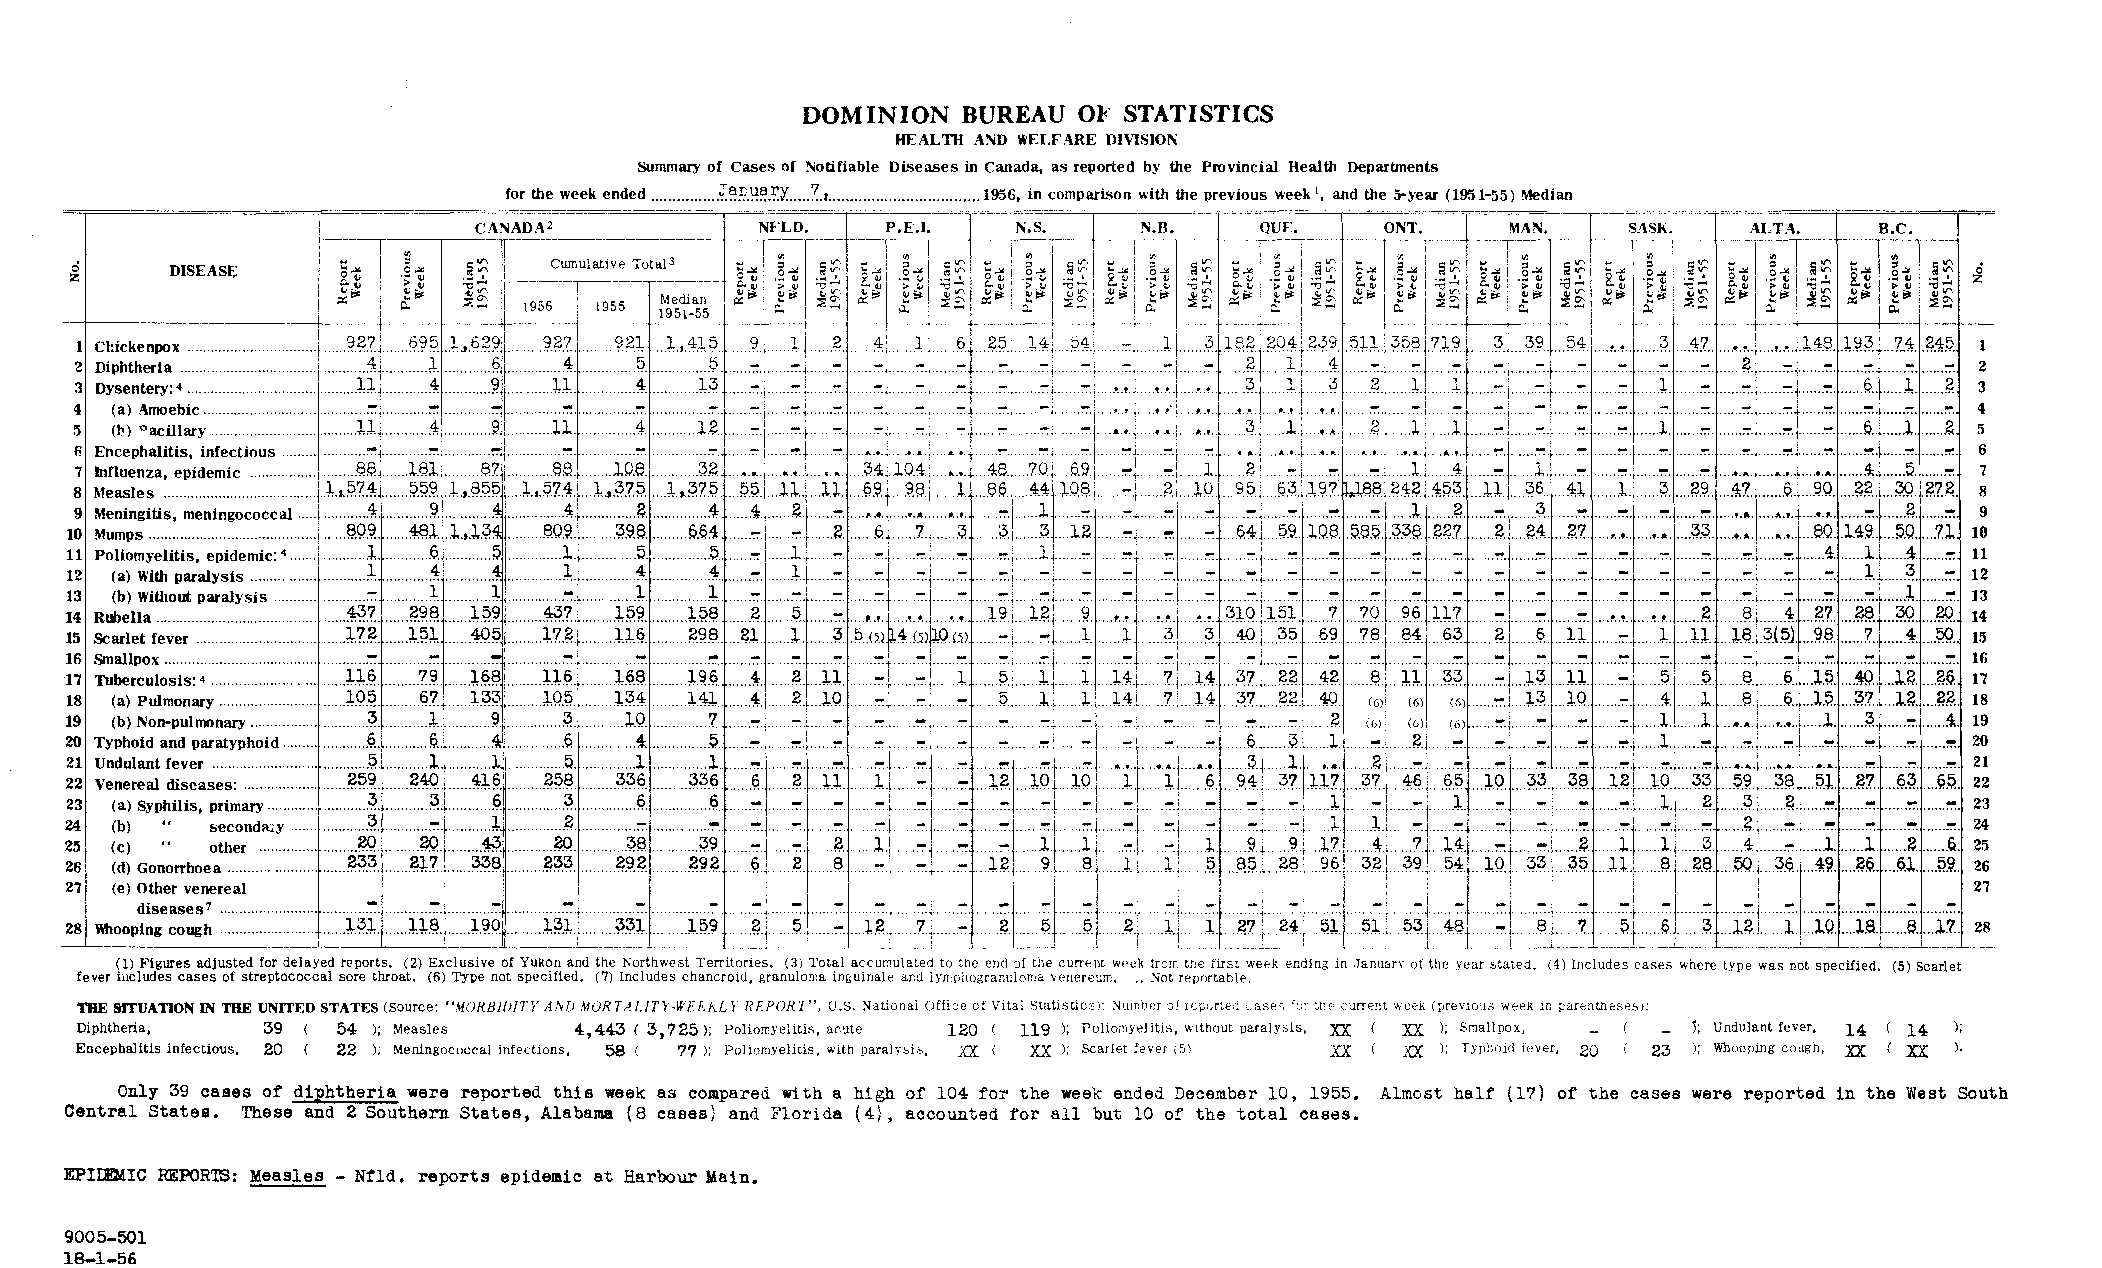
\includegraphics[width=1\linewidth]{figure/cdi_ca_1956_wk_prov_dbs_Part1.pdf}
    \caption{Week 1 table of the Canadian Disease Incidence Dataset}
    \label{fig:NDD1}
\end{figure}


For a human observer, the table shown in \cref{fig:NDD1} is easily interpretable. However, from the perspective of an OCR engine such as Textract, some problems in the cell contents and structure arise. Below are the common problems seen in the cell structure and content that appear in many historical data documents (and lead to problematic results in \cref{sec:NDD}):

\begin{itemize}
    \item Merged cells: In CANDID, many rows contain merged cells. For instance, the cells listing disease cases for Canada are merged, as are the province names and the header for the cumulative total. As a result, row lengths are inconsistent across the table.
    \item Header values that split the data for the current week, previous week, and median are printed vertically, whereas the rest of the table is printed horizontally.
    \item Where data was missing for the week, the document contains ``..'' as a placeholder.
    \item Where there are no cases, the document contains ``-'' as a placeholder.
    \item There is a lot of information useful for interpreting the data at the bottom of the table. Some cells have parentheses next to them with another number (ranging from 1 to 6) referring to a footnote. These footnotes correspond to how the data was collected, the province/territory they was sampled from, etc. For example, in \cref{fig:NDD1} the value ``5(5)'' is entered for P.E.I. under report week for the row ``Scarlet Fever''. This corresponds to 5 cases of the disease in the province, and the (5) corresponds to the footnote ``Scarlet Fever includes cases of streptococcal sore throat.''
    \item At the bottom of each week's table there is information on data named, ``The situation in the United States''. It is not stored in a tabular format, and was therefore not processed with Textract. This corresponds to Textract's ability to successfully complete sub-task 1 in \cref{sec:intro}. However, this is valuable information that a statistician or researcher might need, so it is important to note that the tool we used did not process these data.
\end{itemize}




\subsection{Quebec Dataset}


Collected and maintained by the Dominion Bureau of Statistics, this dataset from July 1927 to December 1931 contains 4.5 years of data. This data is on communicable disease incidences by county and municipality in Quebec. The data points were provided by individual municipalities or the inspectors of the Provincial Bureaus of Health. This dataset is not a part of CANDID because its data has not been manually entered. The scans have been collected and organized by McMaster's Theoretical Biology group. 


The first detail to note on the Quebec dataset is that the structure of the data changed about halfway through the time series, from two tables per page to just one (see \cref{fig:quebecstructures}). We restricted the analysis to the most recent two years of data, which have consistent structure.

The table is organized so that each row represents a specific geographic unit: first the county, and then the municipalities within that county, providing the location of where cases occurred. The columns correspond to different infectious diseases (e.g., Smallpox, Diphtheria, Scarlet Fever, Typhoid, Measles, Tuberculosis, Influenza), giving the classification of the health conditions being tracked.

\begin{figure}[h]
    \centering
    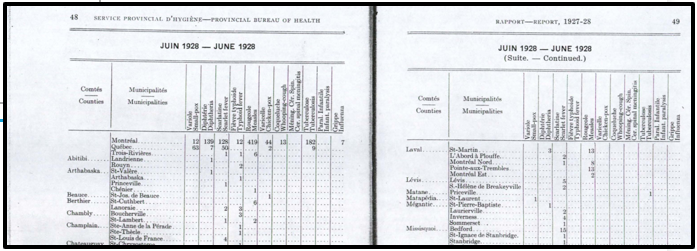
\includegraphics[width=0.8\textwidth]{figure/quebec1.png}
    
    \vspace{0.5cm}
    
    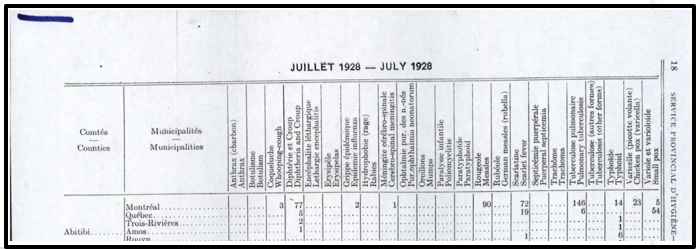
\includegraphics[width=0.8\textwidth]{figure/quebec2.png}
    \caption{Two main table structures from the Quebec dataset.}
    \label{fig:quebecstructures}
\end{figure}

The row headers of the Quebec dataset has row headers are tilted on the diagonal and in French.  This presents challenges also seen in CANDID, such as special characters (i.e. French accents) that now need to be accounted for.

Numeric entries are the count of reported cases for that disease in that municipality during the specified month, while blank cells or dots indicate zero or unreported cases. 




\section{Statistical Measures} \label{sec:measuresAccuracy}

\subsection{Testing Accuracy of Textract Data Compared to Manually Entered Data}
To assess the accuracy of the CANDID data digitized by Textract, we compared it with the corresponding data digitized by humans in McMaster's Theoretical Biology group, using a myriad of metrics.

\subsubsection{Simple Metrics}
The most straightforward measure of accuracy is the percentage of cells from the Textract dataset that are exactly the same as the manual dataset. This is not a measure of cells that were correctly digitized, but rather the proportion of cells whose both content and location (row and column index) are equivalent.

This percent equivalent metric was first applied to the raw extracted data, and then again
as the data became progressively more processed through the methods described in \cref{sec:postprocessing}.

\subsubsection{String Differences and Levenshtein Distance} \label{sec:levdist}
To quantify discrepancies between cells with extracted string and their manually entered counterparts, we compute string-level similarity metrics, with a primary focus on Levenshtein distance \cite{Levenshtein1965BinaryCC}. Levenshtein distance measures the minimum number of single-character edit operations—insertions, deletions, or substitutions—required to transform one string into another. A distance of zero indicates an exact match, while larger values reflect increasing divergence.

Let $s = s_1 s_2 \dots s_m$ and $t = t_1 t_2 \dots t_n$ be two strings of lengths $m$ and $n$. The Levenshtein distance $D(i,j)$ between the characters $s_1 \dots s_i$ and $t_1 \dots t_j$ is defined as follows:
\[
D(0,j) = j \quad \text{for } j = 0,1,\dots,n
\]
\[
D(i,0) = i \quad \text{for } i = 0,1,\dots,m
\]
\[
D(i,j) =
\min \begin{cases}
D(i-1,j) + 1 & \text{(deletion)} \\
D(i,j-1) + 1 & \text{(insertion)} \\
D(i-1,j-1) + \mathbf{1}_{s_i \neq t_j} & \text{(substitution)}
\end{cases}
\]
\[
\mathbf{1}_{s_i \neq t_j} =
\begin{cases}
0, & s_i = t_j \\
1, & s_i \neq t_j
\end{cases}
\]
Finally, the Levenshtein distance between strings $s$ and $t$ is:
\[
\operatorname{Lev}(s,t) = D(m,n)
\]

\cite{wagner1974string} In practice, Levenshtein distance is often normalized by string length to enable fair comparison across tokens of different sizes \cite{Wagner1974}. This is particularly important when evaluating OCR output, where short strings (e.g., years or counts) are disproportionately sensitive to single-character errors.


\subsection{Epidemiologically Significant Statistics Derived from Textract Data}

\subsubsection{Row and Column Sums}
Aggregate counts obtained by summing across diseases or locations are often needed.  If these sums were provided in the original documents, then they also provide a valuable opportunity for consistency checks in the data entry. Thus, it is extremely useful to sum values across a row or down a column and confirm that the result matches the reported total at the end of that row or column. If the sums agree, it provides an immediate check that entries were not missed, duplicated, or mistyped. While it’s technically possible for errors in both the extracted sums and incidence values to cancel out and still agree, this is very unlikely. Discrepancies immediately flag rows or columns that require closer review, allowing errors to be identified and corrected early before downstream analysis.

\subsubsection{Cross-Correlation Between Diseases}
Computing cross-correlation between two disease time series involves measuring how strongly their observed patterns move together over time, and whether changes in one disease tend to occur before, after, or at the same time as changes in the other. Instead of determining whether two diseases are correlated in a broad sense, cross-correlation
examines their relationship across different time shifts. For example, whether peaks in Measles are followed by peaks in Chickenpox one or two weeks later. Mathematically, it compares the standardized values of one time series with shifted versions of the other, producing a correlation value for each lag.

Ordinary correlation measures the linear association between two random variables $X$ and $Y$. 
It is defined as the normalized covariance.
This quantity lies in $[-1,1]$ and measures the strength and direction of linear dependence.

For time series $\{x_t\}$ and $\{y_t\}$, ordinary correlation corresponds to comparing values at the same time index:
\[
\rho_{xy}(0) = 
\frac{\mathrm{Cov}(x_t, y_t)}{\sigma_x \, \sigma_y}.
\]

Cross-correlation extends this idea by introducing a time shift, which is called the lag. 
The cross-covariance at lag $k$ is
\[
\gamma_{xy}(k) = \mathrm{Cov}(x_t, y_{t-k}),
\]
and the cross-correlation function (CCF) is
\[
\rho_{xy}(k) = 
\frac{\gamma_{xy}(k)}{\sigma_x \, \sigma_y}.
\]

Thus, $\rho_{xy}(k)$ is the correlation between $x_t$ and a shifted version of $y_t$. 
By varying $k$, cross-correlation measures linear dependence across different time offsets.

\paragraph{Interpretation:}
\begin{itemize}
    \item $k = 0$: simultaneous association.
    \item $k > 0$: $x$ leads $y$ by $k$ time units.
    \item $k < 0$: $y$ leads $x$ by $|k|$ time units.
\end{itemize}



We will compute the cross correlation function, CCF, $\rho_{xy}(k)$ with $x$ and $y$, referring to two different diseases that were both reported during our time period. Our objective is to compute the CCF using the manually curated data, and then compute the same CCF using the automatically extracted data. This produces two cross-correlation sequences corresponding to the manual and extracted datasets, respectively. If the two CCFs are sufficiently similar, we will conclude that the automatic data extraction is sufficiently accurate to make epidemiologically meaningful inferences.


To assess similarity, we compare these functions across all lags $k$. This can be done by examining differences in (i) the lag at which the maximum correlation occurs, (ii) the magnitude of peak correlations, and (iii) the overall shape of the CCF curves. Quantitatively, one may compute the difference 


\[
\Delta(k) = \rho_{xy}^{\mathrm{M}}(k) - \rho_{xy}^{\mathrm{T}}(k),
\]
where superscripts M and T refer to manual and Textract data, respectively.  If the two CCFs are similar in magnitude, peak location, and overall structure, this suggests that the extracted data preserves the dependence structure present in the manual dataset.


\subsubsection{Other Time Series Statistics}

Another verification tactic is to filter the data by disease---or more generally, by category or type---and examine each subset independently. Analyzing grouped data makes it easier to spot values that are inconsistent with the typical range for that specific group. Outliers can then be identified by visual inspection of scatterplots, boxplots, interquartile range, or standard deviation-based cutoffs.

Using more than one approach reduces the risk of missing meaningful anomalies or over-flagging valid but extreme observations, and helps distinguish true data entry errors from legitimate but rare values.

The test statistics of greatest interest are those that an epidemiologist would be naturally interested in calculating. In a time series of disease incidence, the \emph{peak height} is simply the largest observed value (the maximum number of cases), and the \emph{peak time} is the time index or date at which this maximum occurs. For a time series of a given disease, knowing the peak height and the time at which it occurs is important as it helps predict the intensity of an outbreak. In practice, these can be calculated by scanning the series for the largest value and recording the corresponding time point. 

In the context of analyzing the quality of our extracted data, testing the growth rate is important as it is one of the preliminary statistics that researchers want to know about an epidemic. Estimating the initial growth rate of a disease time series quantifies how quickly the number of cases increases during the early phase of an outbreak. The growth rate provides a concise measure of epidemic speed and can be used to compare outbreaks across locations or time periods. The early phase of an outbreak is typically well-approximated by exponential growth, where the expected number of cases increases proportionally to the current number of cases. The initial exponential growth rate $\lambda$ is particularly important as it yields the epidemic doubling time ($\frac{\ln{2}}{\lambda}$) and can be used to derive quantities such as the basic reproduction number $\mathcal{R}_0$ \cite{WallLips07}.

Methods for estimating the initial exponential growth rate \cite{Ma2014,JaganRpkg} typically take advantage of the fact that if incidence is growing exponentially then cumulative incidence also grows exponentially. Since datasets are often observed at substantial intervals (e.g., weekly), designing methods that use ``interval incidence'' (the difference between cumulative incidence at observation times) is more robust. We can also use the growth rate to calculate the doubling time, which is a statistic that is more easily interpreted numerically.
The exponential growth rate \(r\) is related to the doubling time $T_{\mathrm{d}}$ by
\[
T_{\mathrm{d}} = \frac{\ln 2}{r}
\]

\section{Analyzing the results from the Canadian Disease Incidence Dataset} \label{sec:NDD}
The following section explores the accuracy of table extraction on a particular dataset, namely the Canadian Disease Incidence Dataset (CANDID). 


\subsection{Comparison to Manually Entered Data}
\subsubsection{Simple Metrics}\label{sec:simple}
When comparing values cell by cell for the CANDID tables from 1956, the percentage of cells between the Textract data and manually entered data that were equivalent was 71\%. This is an extremely conservative measure, however, because with additional scripting this jumped to over 97\%. Outlined below are a few interesting ways we modified the Textract data to match the manual data:
\begin{itemize}
    \item Textract produced values in the thousands with a comma, whereas the manual data was not. So $1,000 \neq 1000$ in our original measure. When we considered these values to be the same, the percent accuracy increased to 75\%
    \item We included disease names in the report, however in only considering numbers (numerical values) rather than headers (with letters), the percentage accuracy was 80\%. Of the errors that did occur in the disease names, many were visibly obvious to a human observer. More details on the errors among string values in \cref{sec:levdist}
    \item Some rows were shifted forward by one cell, leading to an entire row returning false. When comparing these values to their shifted index, in an automated process, the accuracy increased to 85\%
    \item Implementing all of the above simultaneously yielded approximately a 97\% match between manual and Textract data
\end{itemize}
\subsubsection{String Differences}
Using Python's NLTK library and its Levenshtein distance function, it is relatively straightforward to find the Levenshtein distance between two strings. The goal is to find the proportion of entries that vary wildly versus not at all. It is illustrative to find the average distance from entries where an actual error occurs. Recall from Section \ref{sec:simple} that 97\% of cell contents are successfully extracted and match the manually entered data, even if they are extracted to the wrong location within a table. The average Levenshtein distance of incorrectly entered data is approximately 2.16. That is to say, given a randomly selected cell extracted with Textract, it is most likely to have two string differences (insertions, deletions, etc) varying from the correct result. Figure \ref{fig:Ldist} shows the proportion of cell contents per Levenshtein distance.

\begin{figure}
    \centering
    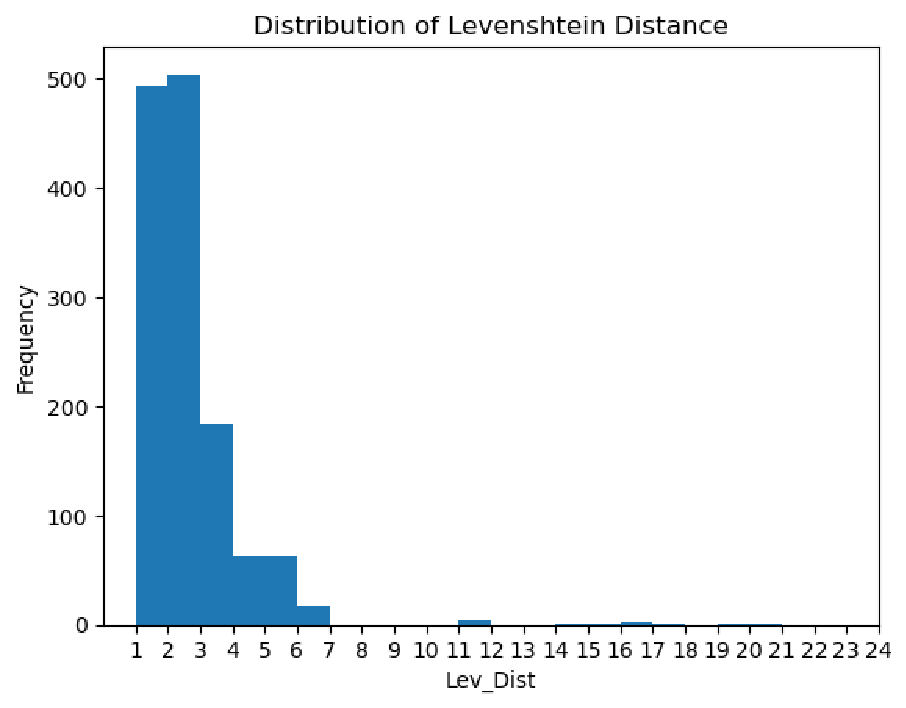
\includegraphics[width=0.7\linewidth]{figure/Lev_dist.pdf}
    \caption{
The frequencies of Levenshtein Distances (defined in \cref{sec:levdist}) between manual and Textract cell values in the CANDID. The majority of distances measured are 1 or 2 differences in characters between the two strings.}
    \label{fig:Ldist}
\end{figure}

We see the most common Levenshtein distances are as expected, namely distances of 1 or 2. This aligns with results from \cref{sec:simple}, where most cell contents differ by a single digit or special character. Of the tables for 1956, between the 1334 cells that we considered to have true extraction errors (i.e. mistakes that were not resolved through post-processing) 37\% have a Levenshtein distance of 1 and 37.8\% have a Levenshtein distance of 2.

The distance value then drops off steadily until it tapers off at a distance of 7. It is likely the OCR engine confuses a blurry part of a number, or that the structure of the table or quality of scan precludes accurate extraction of one or two digits.

The percentage of each Levenshtein distance in cells with errors from the tables for 1956 is seen in \cref{tab:lev_dist}.

\begin{table}[h]
\centering
\begin{tabular}{ccc}
\hline
\textbf{Levenshtein Distance} & \textbf{Count} & \textbf{Percentage} \\
\hline
1  & 493 & 37.0\% \\
2  & 504 & 37.8\% \\
3  & 184 & 13.8\% \\
4  & 63  & 4.7\%  \\
5  & 63  & 4.7\%  \\
6  & 16  & 1.2\%  \\
11 & 4   & 0.3\%  \\
14 & 1   & 0.1\%  \\
15 & 1   & 0.1\%  \\
16 & 2   & 0.1\%  \\
17 & 1   & 0.1\%  \\
19 & 1   & 0.1\%  \\
21 & 1   & 0.1\%  \\
\hline
\end{tabular}
\caption{Distribution of Levenshtein distances between extracted and reference values.}
\label{tab:lev_dist}
\end{table}

There are outliers in the trend seen at a Levenshtein distance of 11, 16 and 21. These errors are almost certainly specific to this dataset and processes. For example, Levenshtein distances of 11 corresponded to the specific errors between the Textract value: ``(e) Other venereal diseases$^{7}$ Whooping cough" and the manual value: ``(e) Other venereal diseases 8". The specific Levenshtein distances, and where they are located, would depend on the structure and content of the table in question. We can expect that longer strings (especially with special characters like those above) would contribute to a larger Levenshtein distance. 

For Levenshtein distances greater than 7, these errors occur exclusively with data corresponding to the names of diseases at the beginning of each row. Again, we can see on row 27 of \cref{fig:NDD1} the cell content corresponding to the disease is ``(e) Other venereal diseases$^{7}$". Extracting this particular cell's contents causes problems for the OCR engine. As described in  \cref{sec:NDDdetails}, this cell value has many problematic characteristics. Its contents span two rows, with the word ``diseases$^{7}$'' appearing below the rest of the disease name. It also has the superscript 7, which is not only much smaller than the rest of the cell contents in the table, but also appears unaligned with the rest of the word. The output from Textract for this cell is ``diseases$^{8}$''. 

Of course, Levenshtein distances of large magnitudes help us in the sense that, following a manual inspection of the extracted data, it would be very clear to a human that an error has occurred. Unlike errors where the Levenshtein distances are 1 or 2, a difference of 20 stands out and would be very simple to manually fix. In addition, distances of this magnitude appear only in entries with character values rather than numeric values. This again means it would be rather simple to fix by a manual reviewer.

We also looked at the relative Levenshtein distance, i.e., the Levenshtein distance proportional to the length of the correct string. This allows us to visualize the errors caused by Textract in a way that accounts for the length of the string
 (see Figure \ref{fig:LdistNormal}). As longer strings have a higher potential Levenshtein distance, normalizing by their lengths aids in determining the proportion of mistakes.
\begin{figure}[H]
    \centering
    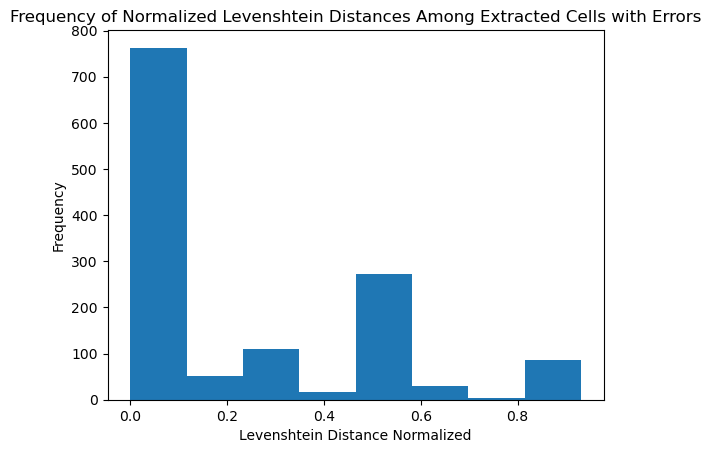
\includegraphics[width=0.7\linewidth]{figure/normalized_L.png}
    \caption{Levenshtein Distance (as defined in \cref{sec:levdist}) normalized by the length of the string of the manually entered cell value.}
    \label{fig:LdistNormal}
\end{figure}
In cells with errors, we see that the most common values of normalized Levenshtein distance is 0.1. 
The other spikes in the graph, around 0.5 and greater than 0.9 can be attributed to shifted cells. For example, when Textract inputs the name of a disease in a cell location that is expected to be a disease count, the character counts between the Textract and manual cell values will vary greatly.
\clearpage

\subsubsection{Detecting Minor Errors with Row Sums}
To mitigate errors arising from row misalignment during extraction, rows corresponding to the same disease were first grouped from each table. Because similar shifting occurs for the same disease in each table, grouping rows by disease prior to checking row sums makes it possible to enforce consistent indexing and ensure that computed quantities are evaluated over the correct set of entries. The structure of the data used for this computation is illustrated in \cref{fig:sumrows}. The total incidence value for the week is in a column titled ``report week'' under ``Canada'' and the contributing cell values similarly appear every third column for each province and territory. 

\begin{figure}[H]
    \centering
    
\includegraphics[width=0.75\linewidth]{figure/computing sums.png}
    \caption{Rows contributing to the computed sums are in blue, and the expected sums are in pink, of the tables in CANDID \cref{sec:NDDdetails}. In the original PDF table, we expect that across a row, the sum of each value in the blue columns equals the total in pink.}
    \label{fig:sumrows}
\end{figure}

By disease, we plot the difference between the expected sums, as extracted by Textract, and the actual sum calculated by looping over the row contents. Below are the values calculated for Measles (see \cref{fig:chickenpoxsum}).

\begin{figure}
    \centering
    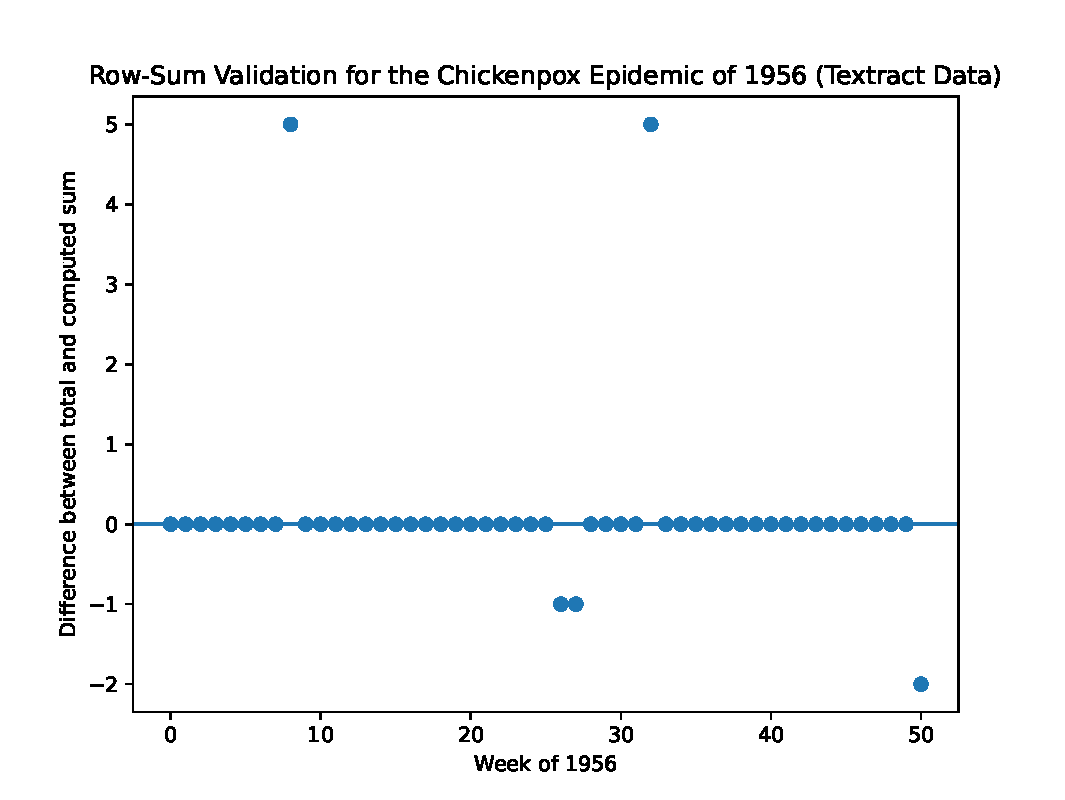
\includegraphics[width=0.7\linewidth]{figure/Chickenpox.pdf}
    \caption{Differences in expected versus calculated row sums for Chickenpox in CANDID (\cref{sec:NDDdetails}) to verify accuracy of cell values (method described in \cref{sec:measuresAccuracy}).}
    \label{fig:chickenpoxsum}
\end{figure}

Most rows exhibit zero difference, indicating agreement between extracted totals and recomputed values. Nonzero deviations indicate inconsistencies that can be traced to numerical errors in individual cells. 



For example, the first outlier in \cref{fig:chickenpoxsum} corresponds to Week 9 in the dataset. From inspecting the scan of the table, we find the true total is \textit{1224}, computed from the non-empty contributing values:

\[55,495,379,25,270\]


In the extracted version of the dataset, Textract correctly extracts the total to be \textit{1224} from the table, but differs on the actual contributing incidents values:

\[50,495,379,25,270\]

Our algorithm found these values and calculated the sum, which is $1,219$. So the difference between the expected sum and the calculated sum is 5, as seen in \cref{fig:chickenpoxsum}. A direct comparison shows that the value 55 was misread as 50. In this way, errors in relatively minor numerical errors can be found and corrected.


Some discrepancies are more subtle. For instance, the first outlier in \cref{fig:measlessum} corresponds to Week 8. The recomputed total from the extracted contributing values is:

\[5,13,59,782,802,61,2,47,111\].


Textract reports a total of \textit{1852}, while the sum of the contributing values equals \textit{1882}. This gives the difference of $-30$ in \cref{fig:measlessum} at week 8. This inconsistency indicates that there exists an error from either the contributing cells or the extraction of the row total, or both. When we compared these values to the scanned document to find the incorrect cells values, the only difference we found was in the cell for the row total, which was manually entered to be \textit{1862} (see \cref{fig:1882}). However, this only accounted for a difference of \textit{10} between the total and the contributing values. 

Upon closer inspection of the source image, the correct value in the scan of the total is \textit{1882} (exactly the sum of the contributing values). This highlights an error in the manual extraction coming from the ambiguity of the original scan.

\begin{figure}[H]
    \centering
    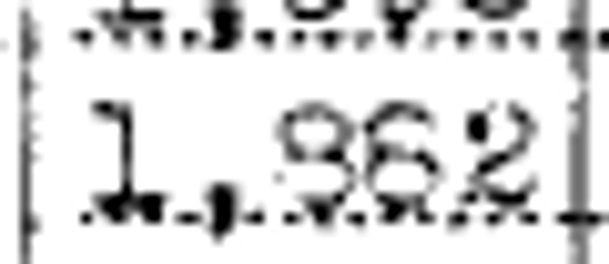
\includegraphics[width=0.10\linewidth]{figure/1882.png}
    \caption{Total Measles instances in Week 9 of CANDID. This is hard to interpret for both OCR and humans.}
    \label{fig:1882}
\end{figure}

These examples illustrate an important advantage of the row-sum validation approach: it detects small inconsistencies in numerical cell contents, and this approach can be adapted for the detection of OCR errors. By comparing independently computed totals with reported values, the method provides a mechanism for flagging anomalies in the dataset.
\begin{figure}
    \centering
    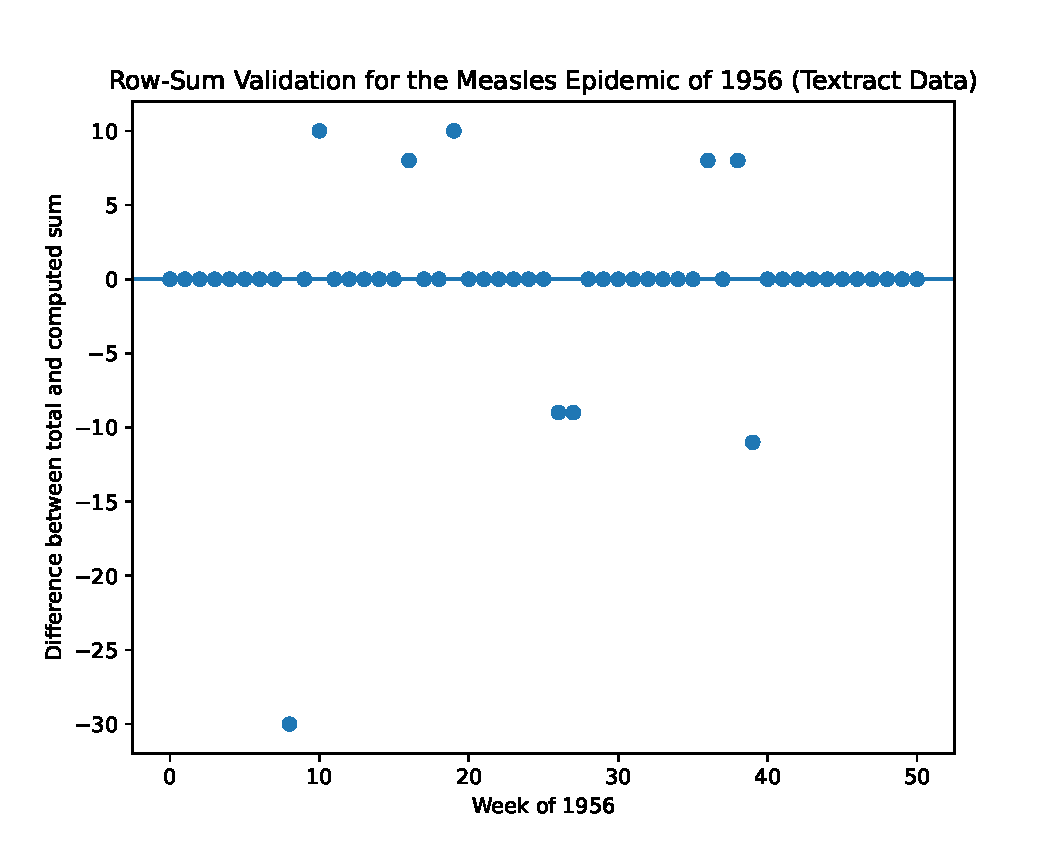
\includegraphics[width=0.7\linewidth]{figure/Measles.pdf}
    \caption{Differences in expected versus calculated row sums for Measles in CANDID (\cref{sec:NDDdetails}) to verify accuracy of cell values (method described in \cref{sec:measuresAccuracy}).}
    \label{fig:measlessum}
\end{figure}

\clearpage
\subsection{Comparing Important Statistics}

\subsubsection{Cross-Correlation Between Diseases} 

The cross-correlation analysis presented first focuses on the relationship between Chickenpox and Measles epidemics. This involved extracting the relevant time series from both the manually curated dataset and the Textract extraction, followed by post-processing to align formats, handle missing values, and ensure consistent indexing across both sources (see \cref{sec:postprocessing}).

To provide an initial qualitative assessment of the relationship between these diseases, and to evaluate the accuracy of the extracted data, we plot the time-series of both datasets \cref{fig:comparisonIncidents}. Visually, the two series are highly similar, indicating that the extraction process preserves the overall timing structure of the data. 

This observation is consistent with the quantitative results reported in \cref{sec:simple}, where it was established that approximately 97\% of values are extracted correctly, with most remaining errors involving only small numerical deviations. As a result, the dominant trends, seasonal patterns, and relative magnitudes of the two diseases are largely unaffected by extraction noise. The remaining 3\% does change the graphs slightly. At around month 60, there is a sharp decrease in Chickenpox, and around month 145, there is some Measles data missing. This is also unsurprising to see in the Textract data, which contains errors that are random and sharp.





\begin{figure}[h!]
    \centering
    
    \begin{subfigure}[b]{0.48\textwidth}
        \centering
        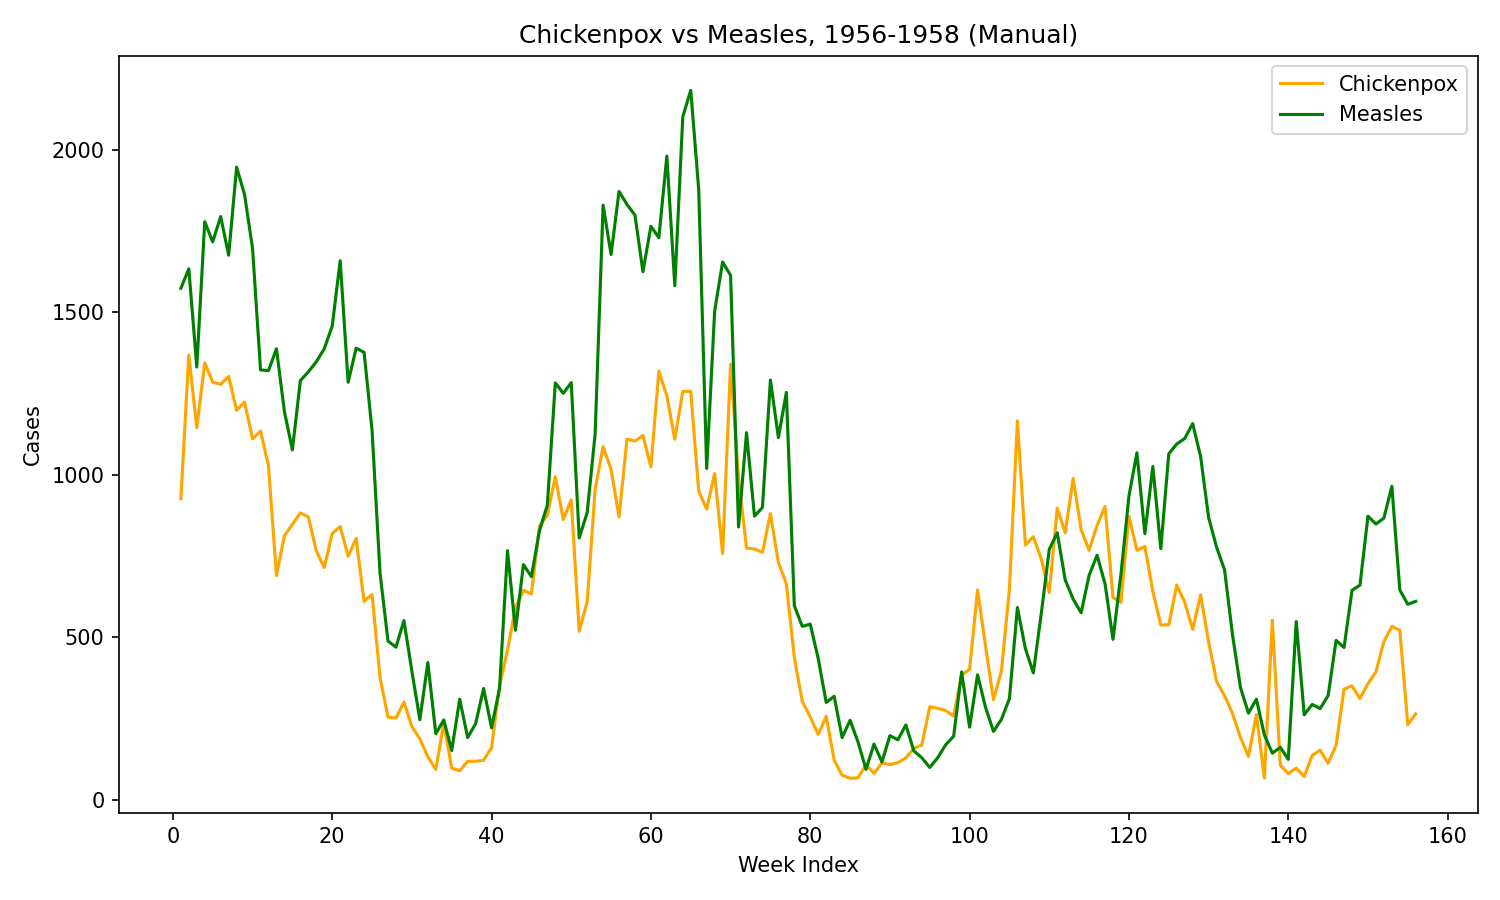
\includegraphics[width=\textwidth]{figure/MeaslesvsChickenpoxmanualdata.png}
        \label{fig:manual}
    \end{subfigure}
    \hfill
    \begin{subfigure}[b]{0.48\textwidth}
        \centering
        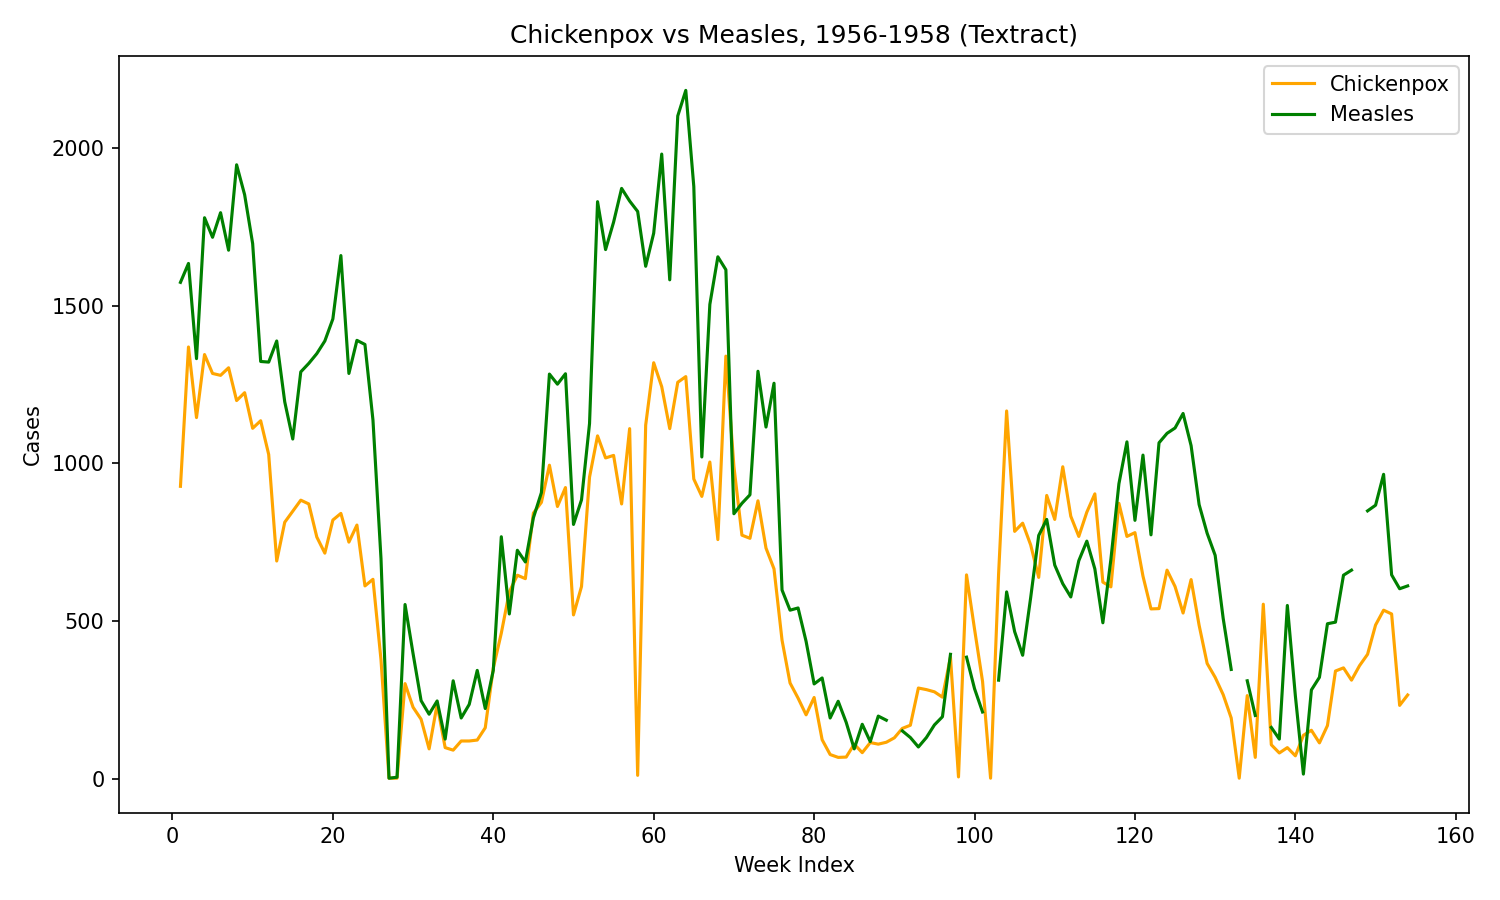
\includegraphics[width=\textwidth]{figure/MeaslesvsChickenpoxtextract.png}
        \label{fig:textract}
    \end{subfigure}
    
    \caption{Comparison of manual versus Textract disease incidence for Chickenpox and Measles.}
    \label{fig:comparisonIncidents}
\end{figure}

The two series rise and fall in roughly the same seasonal pattern, with major peaks and troughs occurring at approximately the same times. Thus, from the incidence curves alone, we would expect a fairly strong positive cross-correlation at lag 0. The cross-correlation function would likely show its maximum at or very near lag 0, with a value that is moderately high after standardization.

For our purposes, it is critical to examine the difference between the cross-correlation computed between the manual and Textract data. The graphs for both computations are shown in \cref{fig:comparisonCrossCorrelation}. These graphs are extremely similar.

\begin{figure}[h!]
    \centering
    
    \begin{subfigure}[b]{0.48\textwidth}
        \centering
        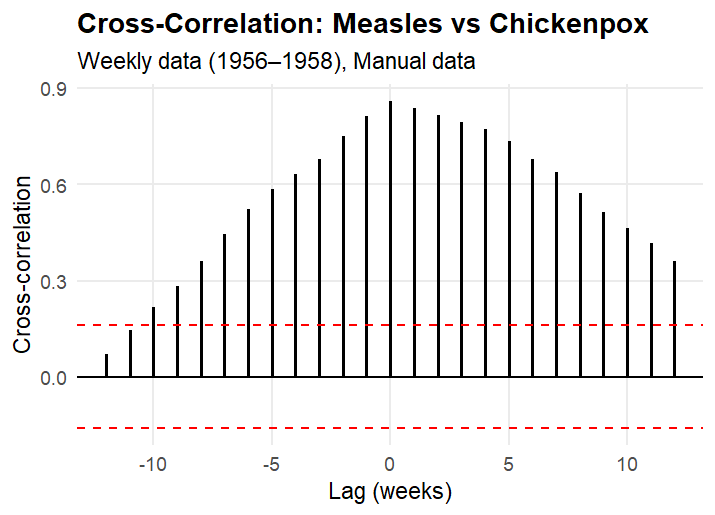
\includegraphics[width=\textwidth]{figure/Cross-correlationMCmanual.png}
    \end{subfigure}
    \hfill
    \begin{subfigure}[b]{0.48\textwidth}
        \centering
        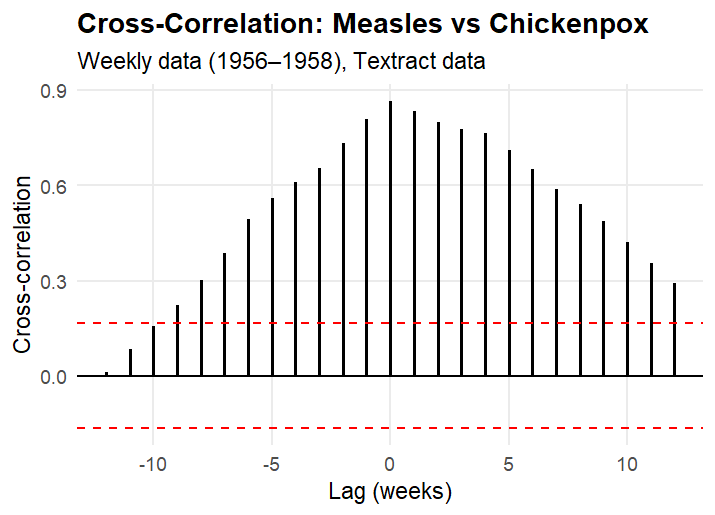
\includegraphics[width=\textwidth]{figure/Cross-correlationMCtextract.png}
    \end{subfigure}
    
    \caption{Comparison of manual versus Textract disease cross-correlation for Chickenpox and Measles. This is described in \cref{sec:measuresAccuracy}.}
    \label{fig:comparisonCrossCorrelation}
\end{figure}

To gain a sense of how similar the cross-correlations are, we computed the differences between them across each lag (see \cref{table:ccdif}).

The strongest correlation occurs at lag 0 in both datasets with a negligible relative difference at the peak ($-0.006$). Across nonzero lags, the Textract correlations are consistently slightly lower than the manual correlations, with relative differences generally ranging from 0.02 to 0.07. Importantly, the lag with the highest cross-correlation remains unchanged, demonstrating that Textract does not distort the timing structure of the series. Because cross-correlation is a measure of time relationships rather than exact magnitudes, we see that the Textract data performs well.

We repeat this process with the time series for Measles and Meningitis (see \cref{fig:comparisonCrossCorrelation2}), and compare the values (see \cref{table:ccdif2}). The CCF graphs are less similar to each other than the Measles and Chickenpox comparison. Note that the Meningitis data required additional post-processing in the form of removing visible outliers (see \cref{sec:hardcoding} below).


\begin{figure}[H]
    \centering
    
    \begin{subfigure}[b]{0.48\textwidth}
        \centering
        \includegraphics[width=\textwidth]{figure/Measles vs Meningitis manual.png}
        \label{fig:manualMM}
    \end{subfigure}
    \hfill
    \begin{subfigure}[b]{0.48\textwidth}
        \centering
        \includegraphics[width=\textwidth]{figure/Measles vs Meningitis textract (hardcoded).png}
        \label{fig:textractMM}
    \end{subfigure}
    
    \caption{Comparison of manual versus Textract disease incidence for Measles and Meningitis. The Meningitis data went through additional postprocessing (\cref{sec:hardcoding}). The Meningitis data without this additional step is seen in \cref{fig:meningitiscomparison}.}
    \label{fig:comparisonIncidentsMM}
\end{figure}

The cross-correlation between Measles and Meningitis is weak across all lags in both the manual and Textract datasets, with values generally between about $-0.11$ and $0.09$. Overall, the same general pattern appears in both datasets. At negative lags, the manual correlations are usually slightly higher than the Textract ones, with the largest differences around lags $-7$ and $-6$ months, where Textract becomes negative while the manual values remain positive.

Around lag 0 and small positive lags (1--4 months), the two datasets are very similar, both showing small positive correlations with only minor differences. At larger positive lags, correlations in both datasets trend toward zero or slightly negative values, though Textract is closer to zero at lags 9 and 10. In short, Textract captures the overall cross-correlation pattern well, and most differences occur where the correlations are already very small.


\begin{table}[h]
\centering
\begin{tabular}{rrrrr}
\toprule
Lag & Manual & Textract & Difference & Relative Difference \\
\midrule
-12 & 0.0710 & 0.0121 & 0.0589 & 0.8296 \\
-11 & 0.1472 & 0.0838 & 0.0634 & 0.4306 \\
-10 & 0.2187 & 0.1581 & 0.0606 & 0.2771 \\
 -9 & 0.2841 & 0.2214 & 0.0627 & 0.2206 \\
 -8 & 0.3621 & 0.3030 & 0.0591 & 0.1632 \\
 -7 & 0.4439 & 0.3870 & 0.0569 & 0.1282 \\
 -6 & 0.5214 & 0.4922 & 0.0293 & 0.0562 \\
 -5 & 0.5862 & 0.5585 & 0.0277 & 0.0473 \\
 -4 & 0.6308 & 0.6108 & 0.0200 & 0.0317 \\
 -3 & 0.6781 & 0.6543 & 0.0238 & 0.0351 \\
 -2 & 0.7497 & 0.7339 & 0.0158 & 0.0211 \\
 -1 & 0.8128 & 0.8095 & 0.0032 & 0.0039 \\
  0 & 0.8600 & 0.8659 & -0.0059 & -0.0069 \\
  1 & 0.8380 & 0.8343 & 0.0036 & 0.0043 \\
  2 & 0.8146 & 0.7992 & 0.0154 & 0.0189 \\
  3 & 0.7926 & 0.7762 & 0.0165 & 0.0208 \\
  4 & 0.7705 & 0.7637 & 0.0067 & 0.0087 \\
  5 & 0.7337 & 0.7102 & 0.0235 & 0.0320 \\
  6 & 0.6788 & 0.6506 & 0.0282 & 0.0416 \\
  7 & 0.6369 & 0.5865 & 0.0503 & 0.0790 \\
  8 & 0.5737 & 0.5423 & 0.0314 & 0.0547 \\
  9 & 0.5136 & 0.4873 & 0.0263 & 0.0512 \\
 10 & 0.4622 & 0.4201 & 0.0421 & 0.0911 \\
 11 & 0.4155 & 0.3553 & 0.0602 & 0.1449 \\
 12 & 0.3608 & 0.2917 & 0.0691 & 0.1915 \\
\bottomrule
\end{tabular}
\caption{Cross-correlation comparison between manual and Textract series with relative differences (Measles vs.\ Chickenpox).}
\label{table:ccdif}
\end{table}




\begin{figure}
    \centering
    \includegraphics[width=0.5\linewidth]{figure/Meningitis manual vs textract.png}
    \caption{Manual (blue) and Extracted (Orange) timeseries for Meningitis. These time series are fairly similar, and this Textract data is plotted \textit{after} the additional postprocessing seen in \cref{sec:hardcoding}}
    \label{fig:meningitiscomparison}
\end{figure}



\begin{table}[h!]
\centering
\begin{tabular}{rrrrr}
\toprule
Lag & Manual & Textract & Difference & Relative Difference \\
\midrule
-12 &  0.062968 &  0.061971 &  0.000997 &  0.01583 \\
-11 &  0.047224 &  0.080284 & -0.033059 & -0.70002 \\
-10 &  0.049490 &  0.064758 & -0.015268 & -0.30851 \\
 -9 &  0.086224 &  0.059327 &  0.026897 &  0.31194 \\
 -8 &  0.070569 &  0.008612 &  0.061957 &  0.87802 \\
 -7 &  0.070657 & -0.040180 &  0.110836 &  1.56851 \\
 -6 &  0.017533 & -0.060253 &  0.077786 &  4.43640 \\
 -5 & -0.009599 & -0.029856 &  0.020257 & -2.11032 \\
 -4 &  0.010779 & -0.034089 &  0.044869 &  4.16282 \\
 -3 & -0.009184 & -0.039498 &  0.030314 & -3.29926 \\
 -2 &  0.019460 &  0.004149 &  0.015311 &  0.78679 \\
 -1 &  0.064041 &  0.040571 &  0.023470 &  0.36647 \\
  0 &  0.063084 &  0.031525 &  0.031559 &  0.50027 \\
  1 &  0.040015 &  0.022251 &  0.017763 &  0.44391 \\
  2 &  0.067676 &  0.053175 &  0.014501 &  0.21427 \\
  3 &  0.079634 &  0.053832 &  0.025802 &  0.32398 \\
  4 &  0.054903 &  0.050776 &  0.004128 &  0.07519 \\
  5 &  0.002288 & -0.003386 &  0.005674 &  2.47990 \\
  6 &  0.016666 &  0.015175 &  0.001491 &  0.08946 \\
  7 &  0.015466 &  0.027459 & -0.011993 & -0.77553 \\
  8 & -0.011577 & -0.024048 &  0.012471 & -1.07742 \\
  9 & -0.079225 &  0.001809 & -0.081034 &  1.02283 \\
 10 & -0.068417 &  0.005542 & -0.073958 &  1.08099 \\
 11 & -0.048158 & -0.035671 & -0.012487 &  0.25928 \\
 12 & -0.108587 & -0.067825 & -0.040763 &  0.37540 \\
\bottomrule
\end{tabular}
\caption{Cross-correlation comparison between manual and Textract series (Measles vs.\ Meningitis).}
\label{table:ccdif2}
\end{table}

\begin{figure}[h!]
    \centering
    
    \begin{subfigure}[b]{0.48\textwidth}
        \centering
        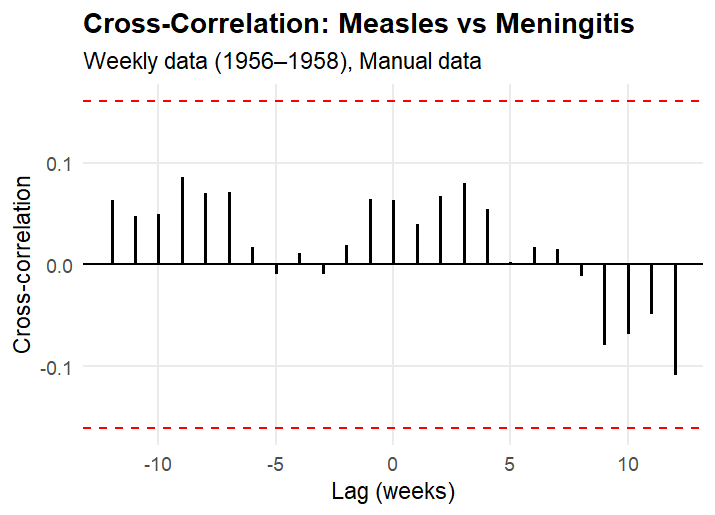
\includegraphics[width=\textwidth]{figure/CCFmanualMM.png}
    \end{subfigure}
    \hfill
    \begin{subfigure}[b]{0.48\textwidth}
        \centering
        \includegraphics[width=\textwidth]{figure/CCFtextractMM(hardcode).png}
    \end{subfigure}
    
    \caption{Comparison of manual versus Textract disease cross-correlation for Measles and Meningitis.}
    \label{fig:comparisonCrossCorrelation2}
\end{figure}

Finally, the same procedure is repeated for a third pair of diseases, namely Chickenpox and Mumps. Time series for both diseases are extracted from the manually curated dataset, and the Textract output, and the corresponding incidence curves are plotted in \cref{fig:comparisonIncidentschM}. Prior to computing the cross-correlation, the extracted data undergoes the same post-processing pipeline used for the Meningitis dataset. In particular, obvious OCR-related errors are identified and manually corrected to ensure that the resulting time series is suitable for analysis. This correction procedure is described in detail in \cref{sec:hardcoding}.


We see in \cref{fig:comparisonCrossCorrelation3} that the graphs of the cross-correlation calculated between Chickenpox and Mumps are very similar between the manual and Textract data. \Cref{table:chickenpoxmeasles} shows that the qualitative differences between the two sets of data at each lag is very small.

\begin{figure}[h!]
    \centering
    
    \begin{subfigure}[b]{0.48\textwidth}
        \centering
        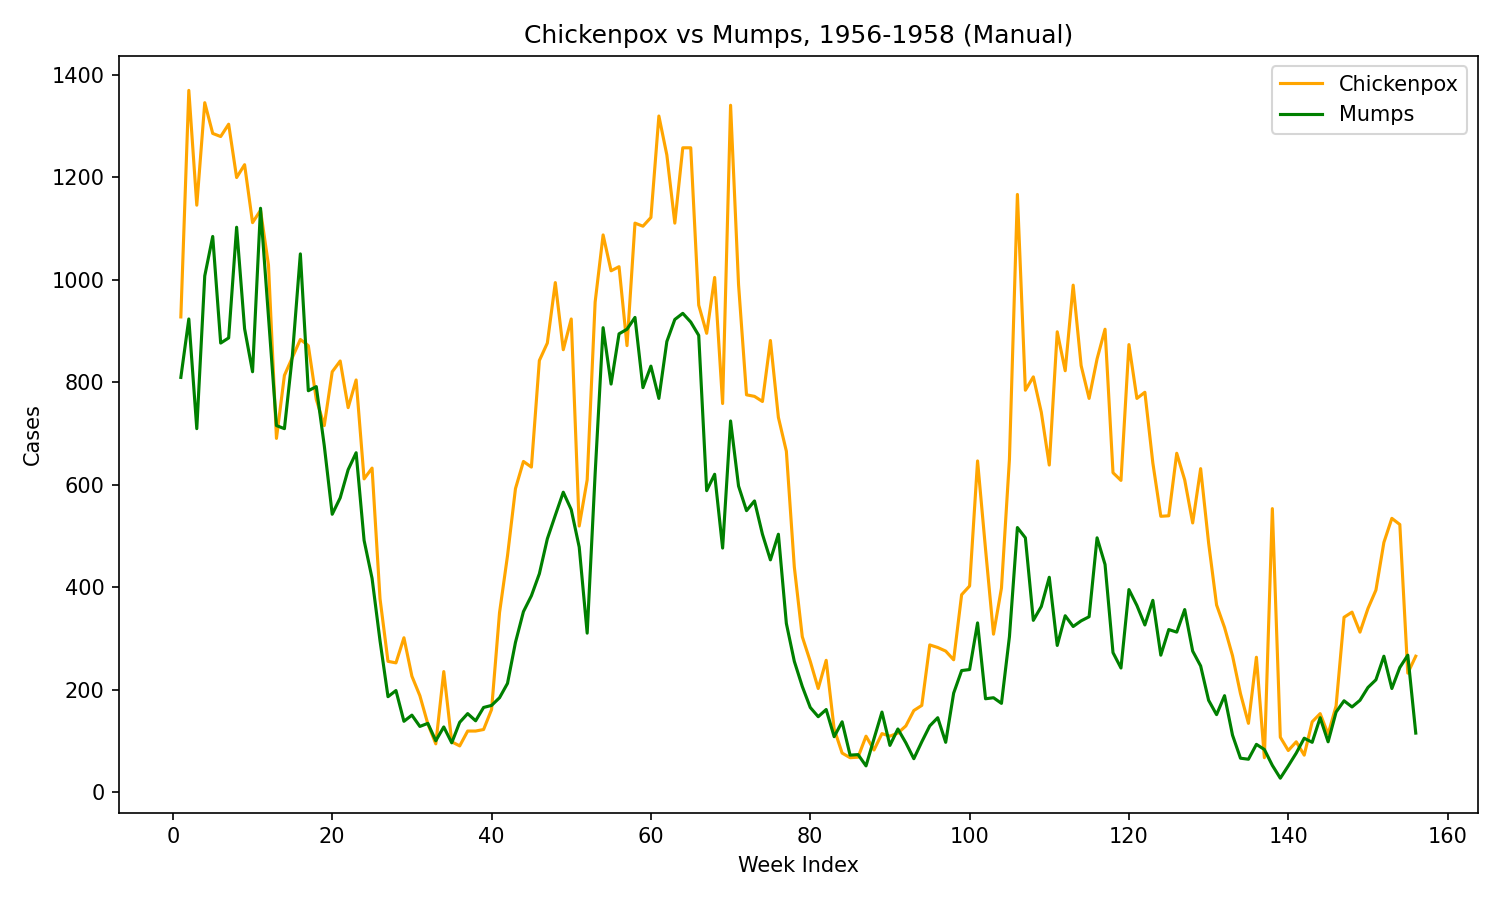
\includegraphics[width=\textwidth]{figure/manual_chickenpox_mumps.png}
        \label{fig:manualchM}
    \end{subfigure}
    \hfill
    \begin{subfigure}[b]{0.48\textwidth}
        \centering
        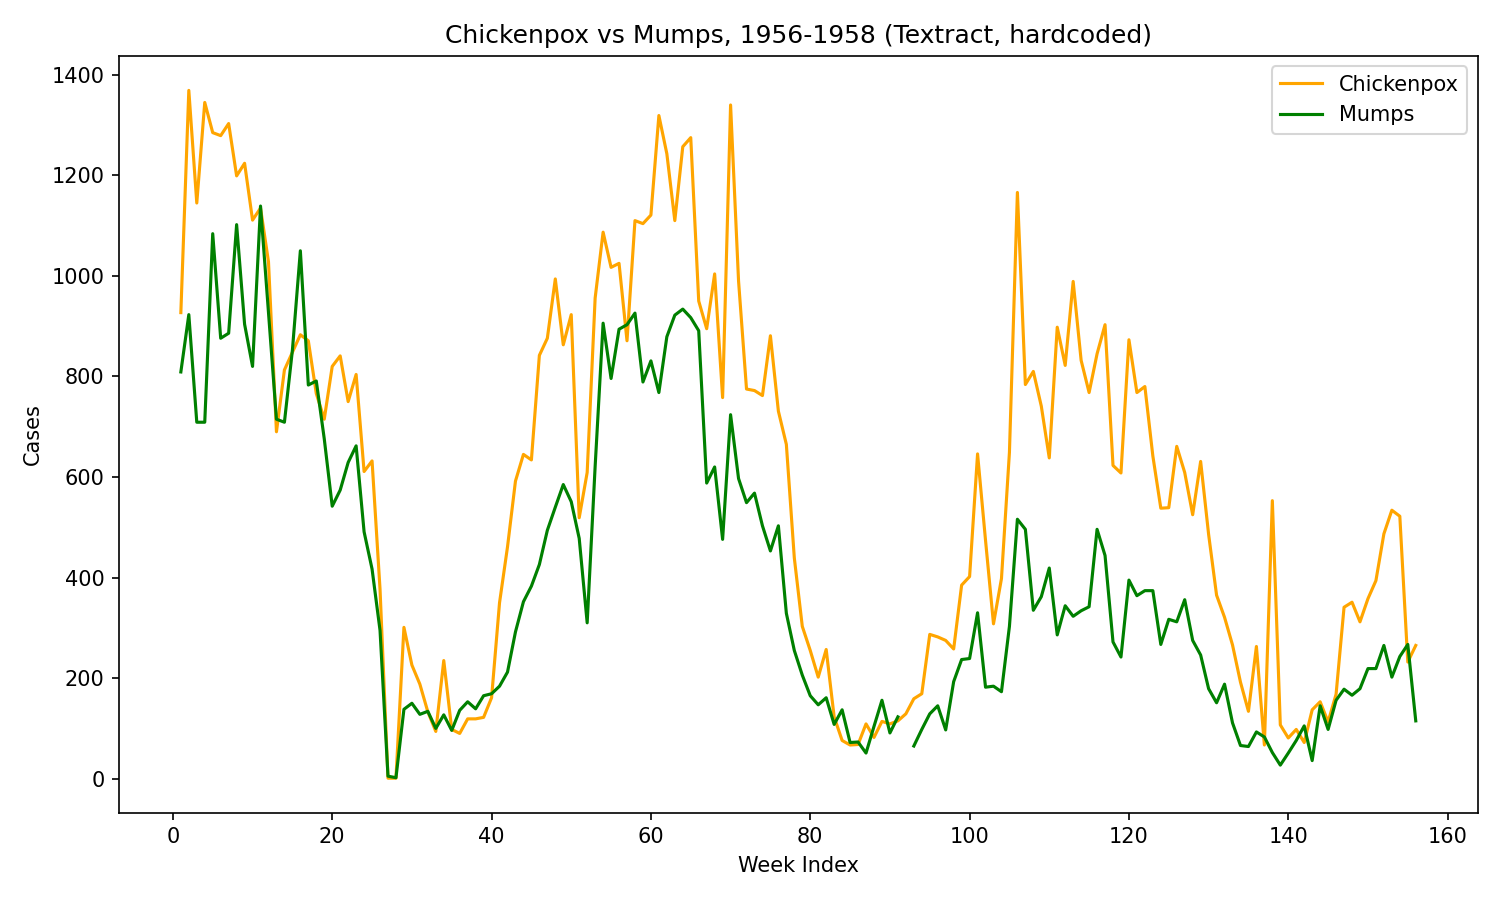
\includegraphics[width=\textwidth]{figure/textract_chickenpox_mumps_hardcoded.png}
        \label{fig:textractchM}
    \end{subfigure}
    
    \caption{Comparison of manual versus Textract disease incidence for Chickenpox and Mumps.}
    \label{fig:comparisonIncidentschM}
\end{figure}

\begin{figure}[h!]
    \centering
    
    \begin{subfigure}[b]{0.48\textwidth}
        \centering
        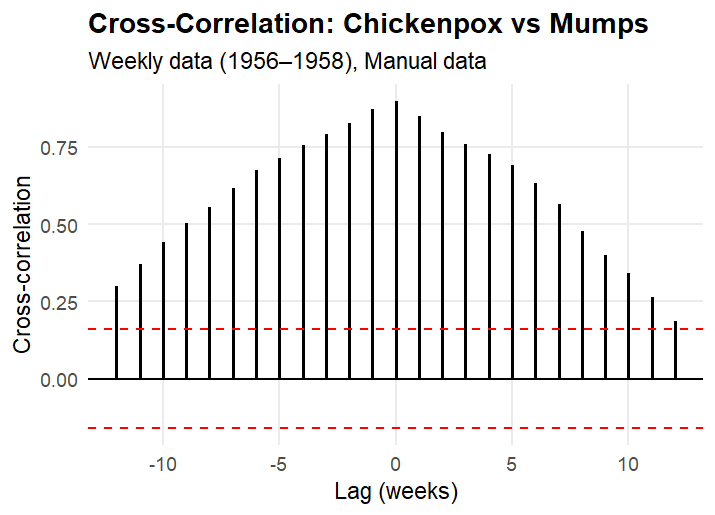
\includegraphics[width=\textwidth]{figure/manualchickenpoxmumpsccf.png}
    \end{subfigure}
    \hfill
    \begin{subfigure}[b]{0.48\textwidth}
        \centering
        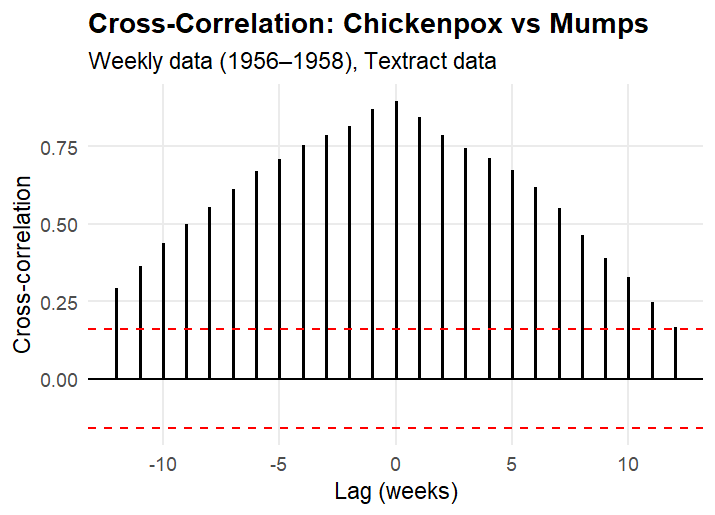
\includegraphics[width=\textwidth]{figure/textractchickenpoxmumpsccf.png}
    \end{subfigure}
    
    \caption{Comparison of manual versus Textract disease cross-correlation for Chickenpox and Mumps.}
    \label{fig:comparisonCrossCorrelation3}
\end{figure}

\begin{table}[h]
\centering
\begin{tabular}{rrrrr}
\hline
Lag & Manual & Textract & Difference & Relative Difference \\
\hline
-12 & 0.2990440 & 0.2918869 & 0.007157094 & 0.02393 \\
-11 & 0.3700199 & 0.3637892 & 0.006230684 & 0.01684 \\
-10 & 0.4427399 & 0.4373411 & 0.005398805 & 0.01219 \\
 -9 & 0.5025446 & 0.4993900 & 0.003154621 & 0.00628 \\
 -8 & 0.5563614 & 0.5534768 & 0.002884684 & 0.00518 \\
 -7 & 0.6161258 & 0.6112137 & 0.004912167 & 0.00797 \\
 -6 & 0.6742270 & 0.6710481 & 0.003178879 & 0.00471 \\
 -5 & 0.7127063 & 0.7081701 & 0.004536180 & 0.00636 \\
 -4 & 0.7570212 & 0.7542702 & 0.002751073 & 0.00363 \\
 -3 & 0.7923939 & 0.7856631 & 0.006730773 & 0.00849 \\
 -2 & 0.8258353 & 0.8145790 & 0.011256294 & 0.01363 \\
 -1 & 0.8714330 & 0.8703313 & 0.001101673 & 0.00126 \\
  0 & 0.8989920 & 0.8974227 & 0.001569220 & 0.00174 \\
  1 & 0.8504960 & 0.8448022 & 0.005693824 & 0.00669 \\
  2 & 0.7992227 & 0.7877855 & 0.011437146 & 0.01431 \\
  3 & 0.7582384 & 0.7448186 & 0.013419830 & 0.01770 \\
  4 & 0.7264547 & 0.7115339 & 0.014920790 & 0.02054 \\
  5 & 0.6898298 & 0.6734192 & 0.016410649 & 0.02378 \\
  6 & 0.6325477 & 0.6177387 & 0.014808954 & 0.02341 \\
  7 & 0.5645311 & 0.5511489 & 0.013382166 & 0.02371 \\
  8 & 0.4762139 & 0.4642939 & 0.011920025 & 0.02503 \\
  9 & 0.3992522 & 0.3895838 & 0.009668385 & 0.02421 \\
 10 & 0.3409900 & 0.3264798 & 0.014510220 & 0.04255 \\
 11 & 0.2642717 & 0.2456713 & 0.018600430 & 0.07038 \\
 12 & 0.1881692 & 0.1676743 & 0.020494854 & 0.10891 \\
\hline
\end{tabular}
\caption{Cross-correlation comparison (Chickenpox and Mumps).}
\label{table:chickenpoxmeasles}
\end{table}

The cross-correlation between diseases and the conclusions we draw from their CCF data is almost identical in both the manual and Textract dataset. In all cases, the peak lag, which is most important for epidemiological study, is identical. All other lags differ very slightly. 



\clearpage

\subsubsection{Time Series Statistics}
After isolating the time series for specific diseases in CANDID, we can find the peak heights and times. In \cref{fig:comparisonIncidents} we can see, in blue, the time series for Measles. As mentioned, the Textract data is very visually similar to the manually entered data. 


The growth rates of the Measles epidemics can be used to calculate the doubling time, which is more meaningful to compare. Both statistics are calculated with the R package \texttt{epigrowthfit} \cite{JaganRpkg}. The graphs below show the doubling time for Measles for both datasets (see \cref{fig:growthratesm}).



We see in \cref{table:measles_growthrate_results} the numeric results from comparing the doubling times, peaks, and peak times between the manually entered and automated datasets.

\begin{figure}[h!]
    \centering
    
    \begin{subfigure}[b]{0.48\textwidth}
        \centering
        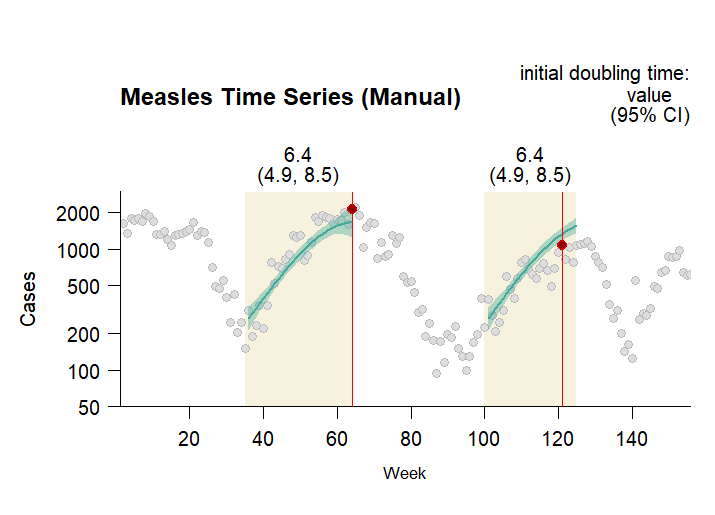
\includegraphics[width=\textwidth]{figure/growthratesmanual.png}
        \label{fig:manualGR}
    \end{subfigure}
    \hfill
    \begin{subfigure}[b]{0.48\textwidth}
        \centering
        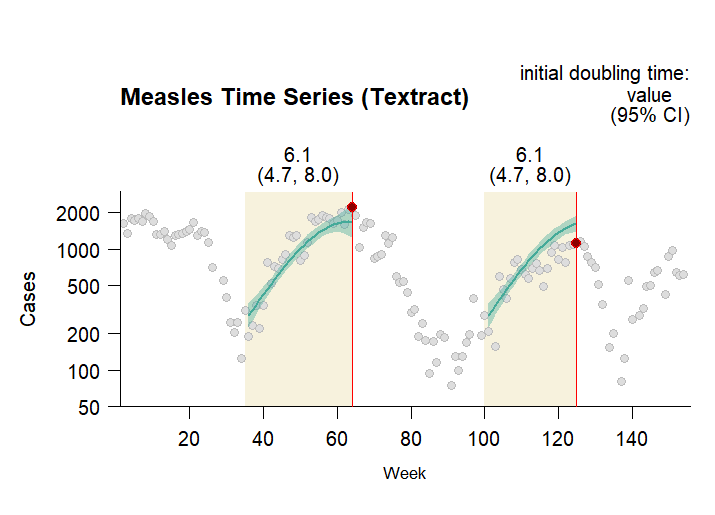
\includegraphics[width=\textwidth]{figure/growratestextract.png}
        \label{fig:textractGR}
    \end{subfigure}
    
    \caption{Manual versus Textract Measles growth rates as described in 
    \cref{sec:measuresAccuracy}.}
    \label{fig:growthratesm}
\end{figure}

\begin{table}[h]
\centering
\begin{tabular}{lcccccc}
\toprule
\textbf{Window} & \textbf{Source} & \textbf{Peak Week} & \textbf{Peak Cases} & \textbf{Week \% Diff} & \textbf{Cases \% Diff} \\
\midrule
Window 1 & Textract & 64  & 2183 & \multirow{2}{*}{0.00\%} & \multirow{2}{*}{3.85\%} \\
         & Manual   & 64  & 2102 &                          &                          \\
\midrule
Window 2 & Textract & 125 & 1112 & \multirow{2}{*}{3.31\%} & \multirow{2}{*}{4.12\%} \\
           & Manual   & 121 & 1068 &                         &                          \\
\bottomrule
\end{tabular}
\caption{Comparison of peak week and peak cases between Textract and manual data with percent differences}
\label{table:measles_growthrate_results}
\end{table}


\begin{figure}[h!]
    \centering
    
    \begin{subfigure}[b]{0.48\textwidth}
        \centering
        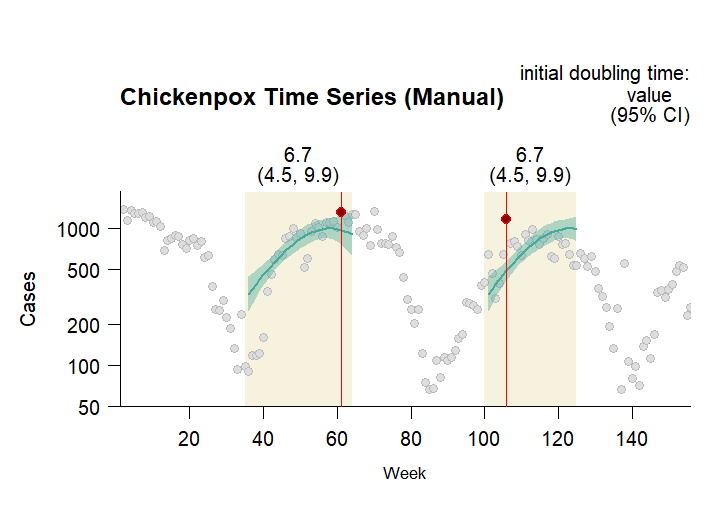
\includegraphics[width=\textwidth]{figure/chickenpox_growth_rate_manual.png}
    \end{subfigure}
    \hfill
    \begin{subfigure}[b]{0.48\textwidth}
        \centering
        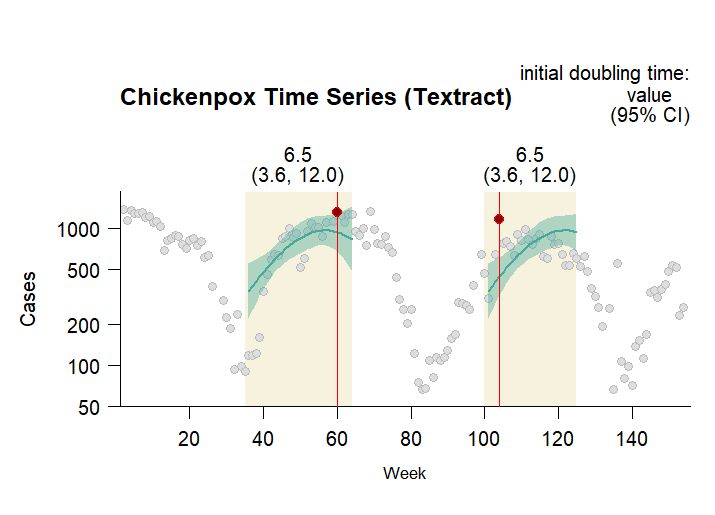
\includegraphics[width=\textwidth]{figure/chickenpox_growth_rate_textract.png}
    \end{subfigure}
    
    \caption{Manual versus Textract Chickenpox growth rates as described in 
    \cref{sec:measuresAccuracy}.}
    \label{fig:growthrateschickenpox}
\end{figure}


\begin{table}[h]
\centering
\begin{tabular}{lcccccc}
\toprule
\textbf{Window} & \textbf{Source} & \textbf{Peak Week} & \textbf{Peak Cases} & \textbf{Week \% Diff} & \textbf{Cases \% Diff} \\
\midrule
Window 1 & Textract & 60  & 1319 & \multirow{2}{*}{-1.64\%} & \multirow{2}{*}{0.00\%} \\
         & Manual   & 61  & 1319 &                           &                          \\
\midrule
Window 2 & Textract & 104 & 1166 & \multirow{2}{*}{-1.89\%} & \multirow{2}{*}{0.00\%} \\
           & Manual   & 106 & 1166 &                          &                          \\
\bottomrule
\end{tabular}
\caption{Comparison of peak week and peak cases for Chickenpox between Textract and manual data with percent differences}
\label{tab:growthrateschickenpox}
\end{table}

We can compare these same statistics with a different disease. For example, \cref{fig:growthrateschickenpox} showcases the doubling times and peaks for Chickenpox as seen in the manual and extracted versions of the dataset. These statistics are compared in \Cref{tab:growthrateschickenpox}.

These very small differences in the epidemiological statistics demonstrate that using Textract data can lead to meaningful results and that Textract data's noise seem unlikely to heavily skew the results of these statistics.


\subsection{Remarks on Dataset Specific Coding}\label{sec:hardcoding}

Several challenges arose when computing row-wise sums for each disease. The primary issue was the extraction errors, such as row misalignment or mislabeled diseases. These issues shifted entire rows of values and consistently propagated across tables, making it difficult to associate values with the correct disease directly. For example, if a disease name contains a comma in the original table, Textract extracts this as two separate cells, shifting the following disease incidence values. As each table has the same or similar disease names, this problem in extraction appeared in each table corresponding to that row. 

Grouping entries by disease (rather than by week as extracted) before performing the summation reduced this complexity. This limited the need for extensive manual intervention, as most diseases had identical errors in each table.

When a shift occurred (typically due to errors in disease labels) the position of the reported total and its corresponding contributing values became offset, and the indices used to identify these values were no longer valid. To address this, the correct indices were re-identified through manual inspection of the extracted data for each disease, and the summation inputs were adjusted accordingly.

An example of this shifting in CANDID occurs with Scarlet Fever. Persistent discrepancies were observed between reported and recomputed sums. Beginning in week 5 of 1956, all row sums appeared incorrect. Investigation revealed that the disease label had changed from ``Scarlet Fever” to ``Scarlet Fever, etc.” in the original document. The introduction of a comma altered the table parsing, causing a shift in all subsequent cell values within the row. This shift propagated through the extraction, leading to misalignment. Resolving this issue required manually identifying the change and recombining the affected cell values to restore the correct structure.

Another key source of error in the row-sum computation arose from the structure of the original tables. In each CANDID table (see \cref{fig:NDD1}), a row index is printed both at the beginning of each row and repeated at the end. Because the summation script iterates over entries at fixed intervals (every third index), these row indices were unintentionally included as part of the contributing values. As a result, the computed sums were systematically inflated. To correct for this, the row index was explicitly identified and subtracted from the computed total (see \cref{fig:hardcode}).



\begin{figure}[h]
\centering
\begin{lstlisting}[language=Python]
for i in range(start_index, len(row), step):
    v = to_int_or_none(row[i])
    if v is not None and v != 8:
        total += v
        used.append((i, v))
\end{lstlisting}
\caption{Part of a Python script to iterate through every third index and manually skip the row value extracted in that row (in this example, this is the $8^{th}$ row).}
\label{fig:hardcode}
\end{figure}
 
We also had to correct extraction errors when comparing the epidemiological statistics between the two datasets. The extracted Meningitis time series contains errors that appear as large, isolated spikes, which are not consistent with the expected disease patterns. Because these errors would distort the results of the cross-correlation analysis, they were corrected before proceeding.
The unprocessed time series for Measles and Meningitis is shown in \cref{fig:raw meningitis textract}. The Measles data follows a smooth and expected pattern, while the Meningitis data includes several sharp spikes that do not match the original dataset. These spikes are caused by OCR errors, where some values are misread or incorrectly extracted.

The following is another example of the Textract time series for Mumps versus Chickenpox, before our manual correction (see \cref{fig:mumpsraw}).

\begin{figure}[H]
    \centering
    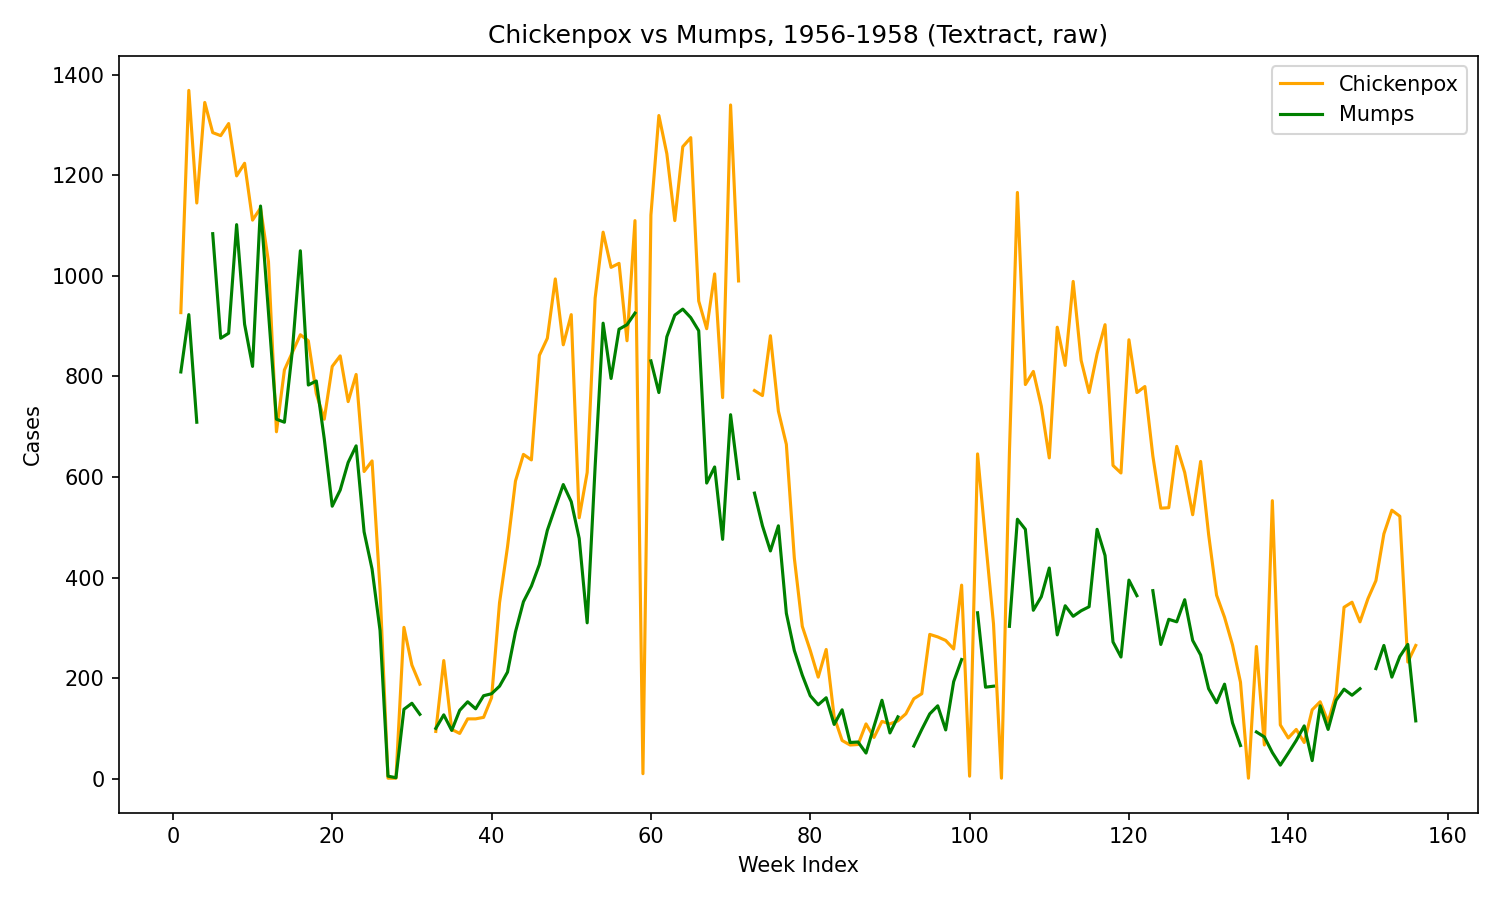
\includegraphics[width=0.7\linewidth]{figure/textract_chickenpox_mumps.png}
    \caption{  The time series for Chickenpox and Mumps from Textract, with clear errors seen around weeks 60, 100, 110, etc as well as missing values.}
    \label{fig:mumpsraw}
\end{figure}


Although these errors are large, they occur only occasionally and are easy to spot. A simple way to identify them is by using a boxplot or violin plot (see \cref{fig:menboxplot}), which clearly highlights these extreme values compared to the rest of the data. This makes it straightforward to locate and verify the errors.

Correcting these incidence values by checking against the original dataset took less than 20 minutes for three years of weekly data. In comparison, manually entering all of this data would take several hours. This shows that, even with some corrections required, the extraction process still saves a significant amount of time.

\begin{figure}[H]
    \centering
    \includegraphics[width=0.5\linewidth]{figure/Measles vs Meningitis no hardcoding.png}
    \caption{Raw Textract values with clear errors in the meningitis cases.}
    \label{fig:raw meningitis textract}
\end{figure}

\begin{figure}[h!]
    \centering
    
    \begin{subfigure}[b]{0.48\textwidth}
        \centering
        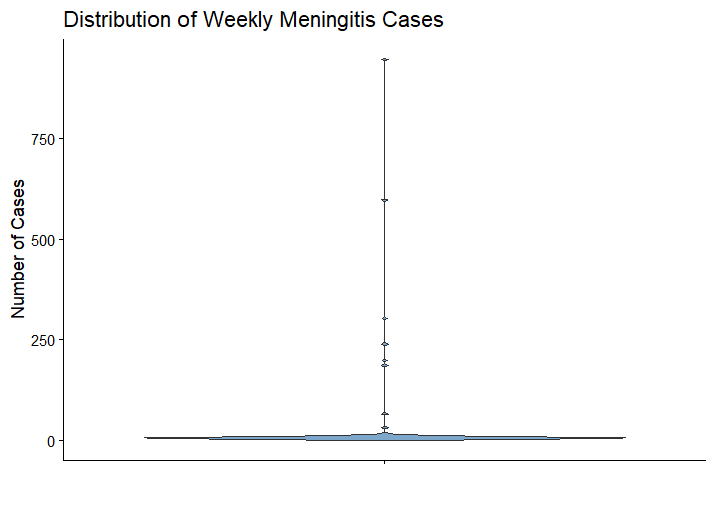
\includegraphics[width=\textwidth]{figure/violin_meningitis.png}
        \label{fig:menboxplotA}
    \end{subfigure}
    \hfill
    \begin{subfigure}[b]{0.48\textwidth}
        \centering
        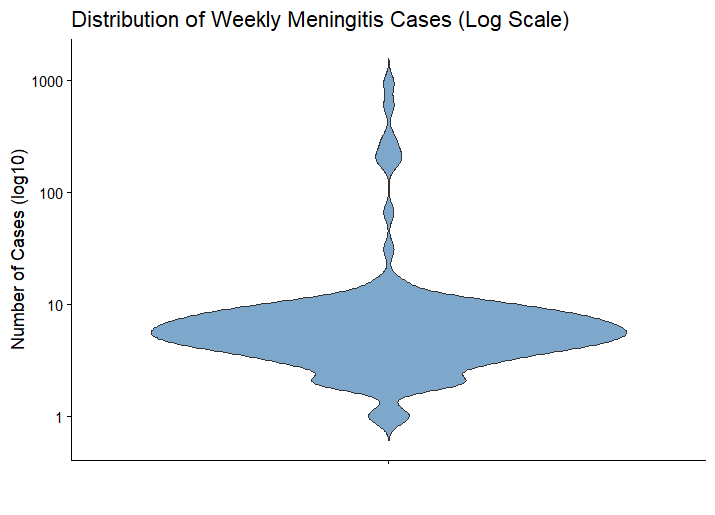
\includegraphics[width=\textwidth]{figure/violin_meningitis_log.png}
        \label{fig:menboxplotB}
    \end{subfigure}
    
    \caption{Violin plots of Textract Meningitis data shown on linear (left) and log (right) scales.}
    \label{fig:menboxplot}
\end{figure}





\clearpage

\section{Conclusion}


\subsection{Impact}
From the perspective of epidemiology researchers, automating tabular data entry is a major aid in studying historical data. It accelerates the processing of large datasets and frees effort and resources for interpretation rather than manual transcription. Because historical sources are often vast, messy, and inconsistent, automation makes it possible to standardize and analyze them at scale, revealing patterns and insights that would have been implausible to uncover in the same amount of time with only manual data entry.

For an automation tool to successfully improve and accelerate the data entry process, it must meet all or most of the requirements we have set in this paper. That is, the software must be relatively simple to use and produce a dataset that is either 
\begin{enumerate}
    \item Close to the original dataset or
    \item Easy to process and fix the errors it produces
\end{enumerate}
If too much human correction is necessary, the time saved becomes relatively small, so the tool is not successful. As well, even with modest time saving, data correction is a less pleasant task for humans than data entry. Even with attempts at automation that were faster than manual entry, the errors were so prevalent and tedious to fix that the tools were ultimately abandoned. As such, our previous attempts to automate the data entry process (for example, with ChatGPT \cite{stewart}) have not met the standards we have outlined above. 

In comparison, the errors present in Textract's table extraction are shown to be of a different character than the inevitable manual entry errors. Textract's errors are often either extremely minute and have a small influence on various statistical tests on the dataset, or so egregiously large and obvious that detection is clear and resolution is easy. This second type of error is also relatively rare and often present in the extraction of string values, which are easy and simple to correct. 

Beyond the initial technical hurdle of utilizing AWS Textract programmatically, as well as the unique post-processing necessary for each dataset, the overall time and effort necessary to recreate CANDID with Textract is reduced in comparison to manual data entry. Similar tables (in both size and complexity) took on average 30 minutes to fully digitize from a scanned copy by a member of McMaster's Theoretical Biology group. If the same rate were achieved for our data from 1956 to 1958, with 156 tables, the manual data entry process would take 78 hours. This is a much longer process than the $\approx15$ minutes our script took to run, and the few hours of writing the necessary scripts for postprocessing. We can therefore conclude that for similar tables, extracting data with Textract can reduce human labour in the data entry process and can be supplemented with dataset-specific post-processing.



\subsection{Limitations}

As our goal was to find a tool that is simple and intuitive to use, we first compared the performance of Textract against an accessible LLM that was not specifically designed for text extraction (specifically, different models of ChatGPT). All table sizes we tested, along with multiple different prompting methods, failed to return extracted data that resembled our scanned document \cite{stewart}. Thus, we limited our investigation to Textract, which we deemed a suitable tool to tackle the three main challenges identified in table extraction after initial experimentation returned data much more similar, visually, to our scanned document. 

The main limitation of Textract is the barrier of entry associated with AWS software. Limited experience with software development might increase the effort required to use Textract. Beyond account set up and writing the extraction script, connecting the code to an AWS account involves an AWS ID, secret key, secret access key and more. However, once the initial setup is complete, researchers have complete control over how the data is processed and extracted. For example, the researcher can choose to omit the confidence levels, certain elements of the table, certain pages of the dataset, etc. In this way, using Textract can more closely model the data entry process. And unlike the data-specific post-processing steps that follow extraction, the same extraction script can be used for any scanned document of a table.

Another limitation is the time required by the software to extract the raw data. For example, the code to extract the CANDID dataset of 156 tables took around 15 minutes to run and terminate. This can be optimized, and time can ultimately be reduced (for instance, by cropping the original datasets to simple parts of the tables). The code that interacts with Textract can itself be optimized by omitting confidence levels and asking the software to extract entire files instead of individual pages of the dataset. There are opportunities for the code and API call to be optimized for better efficiency, but optimizing API calls was not a priority of this project. 


The largest limitation is the time and energy required to process and clean the data post-extraction. This includes the formatting errors of the extracted dataset, such as merged cell errors and shifted row values, as well as finding and correcting the large errors Textract produces in rare numeric values and string headers. By far, this took more time than running the code to extract the data at the onset. However, as mentioned above, this still takes hours less time and effort than manually entering the data by hand. 

Small errors in the extraction process are inevitable and can be particularly difficult to detect, especially when they occur in numerical values that appear plausible at a glance. These errors may arise from OCR misreads, formatting inconsistencies, or noise in the original documents, and they often do not stand out unless carefully validated against source data. It is also important to note that a similar volume of data extraction, even with the modest level of error that occurs before processing, would be impossible to accomplish manually in the same time frame. It would certainly take a human more than 15 minutes to read 156 dense tables, let alone enter the data into a spreadsheet. So while the exact amount of time saved would vary from dataset to dataset, the process of extracting data with Textract reduces the overall time it takes to process scanned documents.

\subsection{Future Work}

Future trials on different datasets will reveal more about the true power and limitations of tools such as Textract. We can expand the scope of our trials to more complicated tables, and to handwritten documents that contain infectious disease data.

Our current results suggest that, even when the initial extraction performs reasonably well on suitable datasets, the bulk of human effort is still concentrated in post-extraction data processing. This includes cleaning inconsistencies, correcting misread values, aligning rows and columns, and validating outputs against source documents. In other words, the main bottleneck is not the extraction itself, but the downstream effort required to make the data usable for analysis.

Going forward, a key objective will be to determine how much of this post-processing stage can be automated. There is strong potential for machine learning tools to play a larger role here. For instance, errors in natural language, such as mislabeled row and column headers that lead to high Levenshtein distances, could be identified and corrected using LLMs trained on domain-specific terminology. Similarly, more sophisticated validation software could be developed to flag anomalies automatically, such as sudden outliers or structural irregularities in tables. These systems could either correct errors directly or generate targeted reports for human review, thereby significantly reducing manual workload while improving consistency and scalability.



\clearpage
\printbibliography 
\end{document}
